\documentclass[a4paper,12pt,oneside]{book}
\usepackage{graphicx}
\usepackage[a4paper, left=2cm, right=2cm, top=2cm, bottom=2cm]{geometry}
\usepackage{tcolorbox}
\tcbuselibrary{listings, skins}
\usepackage{listings}
\usepackage{float}
\usepackage{caption}
\usepackage{tocloft}
\usepackage{hyperref}

\hypersetup{
    colorlinks=true,
    linkcolor=black,
    urlcolor=blue,
    linktoc=all,
    citecolor=blue
}

\title{Fundamentos de GNU/Linux}
\author{Markel Mencía Ramírez}
\date{Enero 2025}


\setlength{\cftsecnumwidth}{3em}  % Increase space for section numbers

\renewcommand{\contentsname}{Índice}
\renewcommand{\chaptername}{Capítulo}
\captionsetup[figure]{name=Imagen}

\usepackage{fontspec}
\setmainfont{RobotoMono-Regular.ttf}[Path=./resources/fonts/, ItalicFont = RobotoMono-Italic.ttf, SlantedFont = RobotoMono-Italic.ttf, BoldFont = RobotoMono-Bold.ttf]
\setmonofont{RobotoMono-Regular.ttf}[Path=./resources/fonts/, ItalicFont = RobotoMono-Italic.ttf, SlantedFont = RobotoMono-Italic.ttf, BoldFont = RobotoMono-Bold.ttf]
\setlength{\parindent}{0pt}
\setlength{\parskip}{1em} 
\renewcommand{\baselinestretch}{1.15}

\lstdefinestyle{mystyle}{
    language=bash,
    keywordstyle=\color{cyan},
    commentstyle=\color{gray},
    stringstyle=\color{orange},
    basicstyle=\ttfamily\footnotesize,
    breakatwhitespace=false,         
    breaklines=true,                 
    captionpos=t,                    
    keepspaces=true,                 
    showspaces=false,                
    showstringspaces=false,
    showtabs=false,
    tabsize=2
}% -- Setting up the custom style:
\lstset{style=mystyle}

\usepackage{tcolorbox}
\newtcolorbox{tcolorbox-code} {
    colback=black!70!gray,
    coltext=white,
    sharp corners
}

\newenvironment{command-info}[5]
{
  \noindent\begin{minipage}{\linewidth}
  \noindent\rule{\linewidth}{1pt}\\[0.5em]
  \noindent{\Large\textbf{#1}}\\[1em]
  \noindent\textbf{Utilidad: }#2\\
  \noindent\textbf{Forma de uso general: }#3\\
  \noindent\textbf{Opciones comunes: }#4\\
  \noindent\textbf{Ayuda: }#5\\
  \noindent\rule{\linewidth}{1pt}\\
  \end{minipage}
}
{
 
}

\begin{document}

\newtcblisting{codeblock}[1][]{
  colback=black!70!gray,
  coltext=white,
  enhanced,
  sharp corners,
  boxrule=0pt,
  listing only,
  listing options={
    language=bash,
    basicstyle=\ttfamily\normalsize\color{white},
    breaklines=true,
    columns=fullflexible,
    keepspaces=true,
    showstringspaces=false,
    keywordstyle=\color{cyan},
    commentstyle=\color{gray},
    stringstyle=\color{orange},
  },
  #1
}

\begin{titlepage}
    \centering
    \vspace*{\fill}
    {\Huge Fundamentos de GNU/Linux\par}
    \vspace{1.5cm}
    {\Large Markel Mencía Ramírez\par}
    \vspace{1cm}
    {\large Enero 2025\par}

    \vfill
    \begin{minipage}{\textwidth}
        \centering
        \raisebox{-0.15\height}{
\includegraphics[height=1em]{resources/images/cc_heart.black.png}}
        {\small 2025. Openly licensed via \href{https://creativecommons.org/licenses/by-sa/4.0/}{CC BY-SA}.\par}
        {\small \href{https://github.com/markelmencia/fundamentos-gnulinux}{Repositorio del libro}\par}
    \end{minipage}
    
\end{titlepage}

\tableofcontents

\chapter{Prólogo}
Este es un curso sobre los Fundamentos de GNU/Linux. En él aprenderás el funcionamiento general del sistema operativo, además del proceso de instalación de éste y el uso de la terminal, una herramienta muy importante para Linux.

El objetivo de este curso no es dominar Linux ni mucho menos. Este curso no intenta ser demasiado teórico ni técnico, la intención es proporcionar herramientas que faciliten al interesado o interesada poder aprender a usar este sistema operativo de forma autodidacta. Para ello, este curso tendrá ejercicios prácticos sobre la terminal para poder aplicar la teoría que se impartirá en estos apuntes. Estos ejercicios se pueden consultar en el repositorio del curso.

Es muy importante recalcar que no entender todo a la primera es normal. A pesar de ser un curso sobre los fundamentos, quizá sea necesario releer apartados y repetir ejercicios lo necesario. Recuerda tomar descansos y preguntar las dudas que necesites resolver. En el \href{https://discord.gg/2qPvfCxD9U}{servidor de Discord de 0xDECODE} estaremos encantados de ayudar.

El autor te anima a que le des una oportunidad a este sistema operativo. Por muy complicado que parezca desde fuera, GNU/Linux es un sistema operativo muy intuitivo y fácil de aprender si te lo propones. Aprenderlo no tiene pérdida, y podría serte de mucha ayuda en un futuro o incluso en la actualidad. No te abrumes si no consigues interiorizar todo el contenido del curso; como he dicho, la intención no es esa, ya que ningún usuario de Linux conoce el sistema de forma completa. Si consigues aprender lo fundamental sobre el funcionamiento de Linux, hasta el punto de poder usarlo de forma cotidiana, este curso habrá cumplido su objetivo.


\textbf{¡Mucha suerte!}
\chapter{Introducción y conceptos básicos}
\section{¿Qué es GNU/Linux?}

GNU/Linux es un sistema operativo enfocado en ser libre, es decir, en que los usuarios tengan la libertad de usar libremente el software sin ningún tipo de licencia privativa.

Es un sistema operativo resultante de décadas de colaboración entre decenas de miles de desarrolladores/as y cientos de empresas. Los dos proyectos principales que forman este sistema operativo son GNU y el kernel de Linux.

\begin{itemize}
\item \textbf{GNU}: GNU es un proyecto de software libre creado por Richard Stallman.
\item \textbf{Linux}: Linux es un kernel creado por Linus Torvalds.
\end{itemize} 

GNU/Linux está basado en otro sistema operativo llamado UNIX, desarrollado por Bell Labs. UNIX, a diferencia de GNU/Linux, no es software libre.

\section{Contexto histórico}
En la década de los 80, ante la creciente privatización que surgió en la industria de la tecnología, Richard Stallman creó el proyecto GNU (GNU's not Unix). El objetivo de este proyecto era conseguir desarrollar un sistema operativo totalmente libre.

GNU desarrolló muchos programas, pero le faltaba un nucleo (o kernel), un componente de un sistema operativo esencial para su funcionamiento.

Linus Torvalds, como proyecto personal, comenzó a desarrollar un kernel que se pudiera unir al software ya creado por el proyecto GNU. Es aquí donde surgió la unión entre estos dos proyectos que hoy conocemos como GNU/Linux.

\textbf{Nota:} GNU/Linux suele ser abreviado por la comunidad a solo "Linux", pero es importante recalcar que una gran parte del software que utilizamos junto con Linux fue creado por GNU, como es el caso de bash, coreutils, gcc, y muchos programas más.

Hoy en día, Linux es utilizado en la gran mayoría de servidores y smartphones del mundo, a pesar de la baja cuota de mercado en ordenadores.

Debido a que es un sistema operativo totalmente gratuito, personalizable, seguro y potente, Linux es un sistema operativo muy aclamado por el mundo de la informática.

\section{Filosofía y valores del Free Software}
Junto con GNU, Richard Stallman creó la Free Software Foundation (FSF), una fundación sin ánimo de lucro con el objetivo de promover el Software Libre. Desde su creación, Stallman y todos los colaboradores/as de la fundación han afirmado que el software libre tiene un impacto más positivo en la sociedad que el software privativo.

Idearon también las cuatro libertades: libertad de Utilizar, Estudiar, Compartir y Mejorar. Estas cuatro libertades son las que necesita ofrecer un software para considerarse libre.

También desarrollaron las licencias "GNU General Public License", unas licencias muy utilizadas en el Software Libre, del tipo "copyleft". Estas licencias se basan en otorgarle al usuario/a las cuatro libertades mencionadas al software que utiliza dicha licencia. Un ejemplo de software que utiliza esta licencia es el kernel de Linux.
Si te interesa saber más sobre la filosofía de la FSF, puedes consultar la página web del proyecto GNU:

\begin{center}
https://www.gnu.org/philosophy/philosophy.html
\end{center}

\section{Componentes clave para Linux}
Linux, como cualquier otro sistema operativo, es un conjunto de componentes diferentes:

\begin{itemize}
    \item \textbf{Bootloader}: Un bootloader es el programa que se encarga de iniciar el sistema operativo al iniciarse el arranque, el proceso de encendido del ordenador. A su vez, el bootloader lo inicia la BIOS/UEFI, un programa almacenado en memoria de solo lectura (ROM) situado en la placa madre de nuestro equipo. Una ventaja de los bootloaders es que gracias a ellos podemos instalar varios sistemas operativos en el mismo ordenador, y acceder a ellos en cualquier momento. Uno de los bootloaders más usados es GRUB, creado por el proyecto GNU.

    \item \textbf{Kernel}: Se le puede considerar el "cerebro" del sistema operativo. Se encarga de enlazar el software con el hardware, y es el componente que se encarga de funciones esenciales como la gestión de memoria, la coordinación del procesador, la conexión entre dispositivos de entrada y salida (E/S o I/O en inglés) y mucho más.

    \item \textbf{Jerarquía de archivos}: Un sistema operativo necesita una forma de organizar sus ficheros (o archivos). En el caso de Linux, es una jerarquía sencilla en forma de árbol. Todos los ficheros y los directorios (carpetas) parten de un solo sitio: / (pronunciado "root", porque es la raíz de la jerarquía). Estos son algunos de los directorios dentro de /:

    \begin{itemize}
        \item \textbf{/bin}: Contiene archivos binarios (ejecutables) de nuestro sistema.
        \item \textbf{/boot}: Contiene los ficheros del bootloader.
        \item \textbf{/etc}: Contiene ficheros de configuración.
        \item \textbf{/dev}: Contiene ficheros relacionados con los dispositivos E/S.
        \item \textbf{/lib}: Contiene las librerías que usa el sistema.
        \item \textbf{/home}: Contiene los directorios de cada usuario.
    \end{itemize}

    	Linux sigue la filosofía "todo es un fichero". Este principio indica que todos los sistemas de funcionamiento dentro de Linux, incluidos los que no tienen que ver con la jerarquía de ficheros, se representan mediante ficheros.

    \item \textbf{Bash (shell), compiladores, y otros programas de GNU}: Son los programas desarrollados por GNU que nos ayudan a interactuar con nuestro sistema. He aquí algunos ejemplos de software creado por GNU:

    \begin{itemize}
        \item \textbf{GNU Compiler Collection (GCC)}: Gracias a él, podemos compilar código de varios lenguajes.
        \item \textbf{GNU C Library (glibc)}: Conjunto de librerías estándar de C que utiliza Linux por defecto.
        \item \textbf{Bash y coreutils}: Conjunto de comandos de terminal.
        \item \textbf{Programas de utilidad varios}: gdb, emacs, wget, tar…
        \item \textbf{Entornos de escritorio}: Son un conjunto de programas que gestionan interfaces para el sistema operativo, y la razón por la que los ordenadores de hoy en día no son solo terminales. Uno de los entornos de escritorio más usado es GNOME, desarrollado por GNU.
    \end{itemize}
\end{itemize}

\section{Distribuciones}
Para facilitar el uso de GNU/Linux, la comunidad ha creado incontables versiones del sistema operativo, cada una con diferentes características y funcionalidades. A estas versiones las denominamos distribuciones. Estas son algunas de las más conocidas:

\begin{itemize}
    \item \textbf{Debian}: Una de las distribuciones más antiguas y más utilizadas por otras distribuciones, como Ubuntu. Debian es conocida por ser muy estable.
    \item \textbf{Fedora}: Distribución basada en incluir las mayores novedades del software libre a su sistema. Es financiada por Red Hat, una compañía que lleva el software libre al mundo empresarial.
    \item \textbf{Arch Linux}: Distribución light muy frecuentemente actualizada. Toda la construcción del sistema depende del usuario/a. 
    \item \textbf{Gentoo}: Sistema muy liberal en cuanto a lo que puedes hacer con el sistema, es muy configurable.
\end{itemize}
\chapter{Instalación de Linux}
\section{Preámbulo}
En estas transparencias se va a mostrar un proceso de  instalación genérico.

Este proceso puede variar en función de la distribución, pero todas las instalaciones requieren configurar muchos de los pasos que vamos a ver.

Normalmente las distribuciones ofrecen un sistema de instalación automático/guiado, pero conocer cómo funcionan las instalaciones por debajo de la interfaz puede ayudarte a comprender mejor el funcionamiento de un sistema operativo.

Es importante recalcar que no comprender todo a la primera es normal. Cuanto más instalaciones hagas, tanto guiadas como manuales, más aprenderás.

\begin{enumerate}
    \item Selección de distribución
    \item Preparación del medio de instalación
    \item Configurar el arranque
    \item Seleccionar tu distribución de tecla, idioma y zona horaria
    \item Crear, formatear y montar particiones de disco
    \item Configurar internet
    \item Instalar los paquetes base de Linux
    \item Instalar entorno de escritorio
    \item Crear usuario
    \item Instalar bootloader
\end{enumerate}

\section{Selección de distribución}
Para seleccionar una distribución, hay algunos factores que debes tener en cuenta:
\begin{itemize}
    \item \textbf{Tu conocimiento sobre Linux}: algunas distribuciones son más complicadas de manejar que otras. Conviene empezar con distribuciones sencillas antes de saltar a unas más complejas.
    \item \textbf{Tus necesidades de software}: Dependiendo de tus necesidades, algunas distribuciones pueden ser más favorables que otras. Por ejemplo, se suele escoger Debian para programar servidores, ya que es una distribución muy estable.
    \item \textbf{El nivel de personalización que necesitas}: Algunas distribuciones te dan más control sobre tu sistema, esto puede ser un factor a tener en cuenta en tu elección.
    \item \textbf{La actividad en el desarrollo de la distribución}: Es recomendable elegir una distribución que esté constantemente en desarrollo por un equipo grande de desarrolladores/as. En caso contrario, tu distribución podría ser más vulnerable a ataques.
\end{itemize}

Si no sabes qué distribución elegir, consulta las más populares. Distribuciones como Ubuntu, Linux Mint o Manjaro son distribuciones muy aptas para gente que está empezando.

\section{Preparación del medio de instalación}
Para instalar un sistema operativo, necesitamos un conjunto de programas que hacen la función de instalador. Estos programas se introducen en un dispositivo de almacenamiento externo para poder ejecutarse en un sistema que no tiene por qué tener "nada".

Para este paso tienes que consultar la página web de la distribución que deseas instalar, y descargar una imagen ISO de instalación.

Un paso opcional pero recomendable es verificar la firma de la imagen ISO. Esto se hace para comprobar que la imagen es legítima y no ha sido infectada con código malicioso. Este paso varía en función de la distro.

Prepara un dispositivo de almacenamiento externo como un flash-drive o un disco óptico. Asegúrate de guardar en otro lugar los datos del dispositivo ya que éste será formateado.

Descarga una utilidad de booteo. Son programas que nos ayudan a convertir nuestro dispositivo de almacenamiento externo en unidades "booteables", es decir, que se pueden ejecutar en el arranque del sistema, como los bootloaders. A este proceso se le llama "flashear".

Una de las utilidades de booteo más utilizadas es Rufus. Es portable, fácil de usar y cumple con su funcionalidad.

\section{Configurar el arranque}
Una vez tenemos nuestro medio de instalación preparado, es hora de configurar el arranque de nuestro sistema para hacer que el programa de instalación se ejecute al encender el equipo.

Para esto tenemos que acceder a la BIOS/UEFI, un programa en almacenamiento de solo lectura (ROM) en nuestra placa madre. Entre otras cosas, la BIOS/UEFI tiene un rol muy importante en el arranque, ya que éste se configura ahí.

En función de la marca de tu ordenador, tu BIOS o UEFI puede ser diferente a otras, pero todas deberían tener opciones de arranque. Consulta en internet como acceder a la BIOS/UEFI y modificar el arranque de tu sistema con tu marca de ordenador.

\section{Seleccionar tu distribución de teclado, idioma y zona horaria}
A partir de este paso comienza la instalación de Linux.

Al haber modificado el arranque para que el equipo se ejecute en tu dispositivo, al reiniciar el sistema accederemos a la instalación.

Normalmente lo primero que se suele configurar es tu distribución o layout del teclado, para poder usar el teclado sin ningún problema durante la instalación.

Una vez configurado el teclado se suele configurar también el locale, un conjunto de datos sobre tu localización como idioma, zona horaria...

\section{Crear, formatear y montar particiones de disco}
Por temas de seguridad y organización, el almacenamiento de nuestro disco duro se divide en áreas para diferentes usos. A estas áreas se les llama particiones.

En Linux se suelen configurar estas particiones principales:

\begin{itemize}
    \item \textbf{Partición / (root)}: Aquí se instala el SO de Linux.
    \item \textbf{Partición /home (opcional pero recomendada)}: Aquí se almacenan tus archivos de usuario (documentos, vídeos...)
    \item \textbf{Partición swap}: Esta partición se usa como "RAM de reserva", cuando agotamos nuestra RAM normal.
    \item \textbf{Partición /boot (opcional pero recomendada)}: Partición pequeña con los programas de arranque.
\end{itemize}

¿Qué es sistema de archivos?: Un sistema de archivos (o filesystem) es un formato que utiliza un sistema operativo para guardar datos. Windows usa NTFS. Linux usa ext4.

Cuando creamos una partición, tenemos que definir su tipo de filesystem o sistema de archivos. Esto es de vital importancia porque si seleccionamos un filesystem equivocado, es posible que Linux no reconozca la partición.

Cada partición mencionada tiene unas características, vamos a verlas una a una:

\begin{itemize}
    \item /boot: Almacena los ficheros y programas de arranque, como el bootloader. Es una partición opcional, pero por temas de compatibilidad con la BIOS y por temas de cifrado en otras particiones, se suele separar de otras particiones.
    \begin{itemize}
        \item \textbf{Tamaño recomendado}: No más de 1GB
        \item \textbf{Filesystem}: Depende del bootloader, pero normalmente por temas de compatibilidad se formatea con FAT32 (que es obligatorio si quieres hacer dual boot  con Windows)
    \end{itemize}

    \item \textbf{swap}: La partición swap es un área del disco duro que reservamos para usarla como "RAM de emergencia". Si por la razón que sea se nos agota nuestra RAM, nuestro disco duro hará de respaldo, a pesar de que el acceso a disco sea mucho más lento. A esta memoria de emergencia se le llama memoria virtual.
    \begin{itemize}
        \item \textbf{Tamaño recomendado}: Depende de tu RAM, y del criterio que desees seguir. Por ejemplo, un criterio que se ha usado mucho tiempo es asignar el doble de gigas de RAM que tengas a la partición swap, pero no siempre hace falta tanto.
        \item \textbf{Filesystem}: "Ninguno", se formatea de una forma especial.
    \end{itemize}

    \item \textbf{/}: Al llamarse / (root), contiene todos los archivos que parten de /, es decir, todos los archivos de nuestro sistema operativo, excepto los de /boot porque creamos una partición diferente para ese directorio.

    \begin{itemize}
        \item \textbf{Tamaño recomendado}: Depende de si vas a crear una partición para /home o no. Si vas a crear una partición para /home, 20-50GB deberían de ser suficientes, pero esto depende de cuántos paquetes vas a instalar en el sistema. Si no vas a crear una partición para /home (ni otras particiones a parte de las mencionadas), asígnale el espacio restante que te queda en disco.
        \item \textbf{Filesystem}: ext4
    \end{itemize}

    \item \textbf{/home}: Contiene tus ficheros personales de tu(s) usuario(s). Es recomendable crear esta partición si te interesa que tus datos sean portables. Si deseas cambiar de distribución, para hacerlo bastaría con eliminar todas las particiones menos la de /home. Así, el sistema operativo se restablecerá para poder instalar otra distribución pero tus ficheros personales permanecerán intactos.

    \begin{itemize}
        \item \textbf{Tamaño recomendado}: Generalmente hablando, a esta partición se le suele asignar el espacio restante que le queda a tu disco una vez has creado el resto de particiones.
        \item \textbf{Filesystem}: ext4
    \end{itemize}
\end{itemize}

\section{Configurar internet}
Necesitamos una conexión a internet para descargar paquetes.

Si tienes Ethernet, no tendrás que configurar nada, pero algunas instalaciones requieren configurar interfaces de red para poder establecer conexiones Wi-Fi.

Si tienes acceso a consola, una forma muy sencilla de comprobar que tienes conexión a internet es mediante el comando ping, que manda paquetes "de prueba" a un dominio para comprobar la conexión. Por ejemplo:

\begin{tcolorbox-code}
\begin{lstlisting}
$ ping google.com
\end{lstlisting}
\end{tcolorbox-code}

\section{Instalar los paquetes base de Linux}
Los paquetes base de Linux son un conjunto de programas y utilidades esenciales para el funcionamiento del sistema operativo.

Para instalarlos, necesitamos saber cuál es el gestor de paquetes de nuestra distribución. Un gestor de paquetes (o packet manager) es el programa que usamos para instalar paquetes en nuestro sistema. Estos paquetes puede ser desde entornos de escritorio enteros como GNOME hasta programas como VS Code.

Cada distro suele tener un packet manager por defecto. En Debian es apt, en distribuciones de Red Hat (como Fedora) es RPM/DNF, en Arch Linux es Pacman.

Cada Packet Manager tiene sus propios paquetes base, con diferentes nombres y características. Eso sí, normalmente todos los Packet Managers ofrecen en sus paquetes base las herramientas más fundamentales de GNU/Linux, como coreutils, bash, systemd, glibc...

Al descargar los paquetes, el mismo Packet Manager se encarga de instalarlos. Además, es importante mencionar que las actualizaciones del sistema también se hacen mediante el Packet Manager. Por tanto, es importante aprender a manejar cómodamente el Packet Manager de tu distribución, ya que es una parte muy importante de éste.

\section{Instalar entorno de escritorio}
Esta parte es opcional pero muy recomendable, sobre todo para las personas que están empezando. Además, hasta los usuarios/as más acérrimos a usar la terminal lo máximo posible tienen un entorno de escritorio, ya que además de ofrecer interfaces, nos facilitan otras funcionalidades de utilidad.

Los entornos de escritorio también se instalan mediante el Packet Manager, y si se hace de forma manual, es posible que requieran configuraciones que no hace el Packet Manager. Sin embargo, la mayoría de distribuciones instalan un entorno de escritorio automáticamente (como muchos de los pasos anteriores).

\section{Crear usuario}
Para leer/escribir/ejecutar archivos, iniciar procesos, gestionar permisos y tener un directorio de trabajo, es necesario tener un usuario.

Linux por defecto viene con un usuario configurado, "root". Este usuario tiene permisos absolutos en el sistema. Sin embargo, por cuestiones de seguridad es recomendable crear un usuario normal por separado que no tenga permisos root. Si queremos hacer una acción que requiera permisos de root, existe el comando "sudo" que, tras introducir la contraseña del usuario root, nos otorga permisos de root en nuestro usuario no-root.

Volviendo a la instalación, antes de crear un usuario nuevo tenemos que otorgarle una contraseña al usuario root (la que tendremos que introducir al usar sudo). Si nuestro instalador no nos ofrece una interfaz para hacerlo, tenemos que usar el comando passwd, y seguir sus instrucciones.

A continuación, tenemos que crear un usuario nuevo. Por norma general esto se hace con el comando useradd, usando luego passwd para establecer una contraseña.
De nuevo, normalmente las instalaciones son guiadas y nos facilitan todo este proceso.

\section{Instalar bootloader}
La instalación está terminada, solo falta instalar un bootloader para que la BIOS/UEFI reconozca el sistema operativo y lo pueda ejecutar en el arranque.

Uno de los bootloaders más usados es GRUB (GRand Unified Bootloader), y es el que eligen por defecto muchas distribuciones como Ubuntu.

Si el instalador no instala GRUB (u otro bootloader) automáticamente, es posible que configuración adicional sea necesaria para configurar correctamente el arranque.

Una vez instalado el bootloader, ya podemos reiniciar el sistema, extraer el medio de instalación, reconfigurar el arranque en la BIOS/UEFI (si es necesario), y reiniciar el sistema.

\chapter{Introducción a la terminal}
\section{Preámbulo}
Saber utilizar la terminal es una habilidad clave para el uso de Linux. Cualquier informático/a que sea capaz de utilizar la terminal de forma eficiente es capaz incluso de sobrepasar la eficiencia de las interfaces gráficas.

A pesar de que parezca lo contrario, aprender a usar la terminal no es una cuestión de memorización, sino de compresión. Es importante conocer cómo funciona Linux como sistema operativo.

Una habilidad muy importante para aprender a usar la terminal (y para cualquier ámbito de la informática realmente) es saber buscar información. Esto significa saber buscar en foros, filtrar información, y saber cómo formular tus dudas en el buscador.

Para terminar, cabe recalcar la importancia de la práctica. La práctica es la clave para dominar la terminal. Usarla lo máximo posible en tu día a día hará que poco a poco te vayas acostumbrando a su funcionamiento. La mayoría de tus habilidades usando la terminal se conseguirán de forma pasiva, haciendo otras actividades o proyectos en ella.

Una forma muy buena de practicar la terminal es simplemente pasarse a Linux. Para empezar puedes configurar tu máquina para que sea dual boot (sistema operativo dual, en este caso tu sistema operativo habitual + Linux), así puedes probar Linux sin necesariamente eliminar tu SO original.

\section{Introducción}
Una terminal es una Interfaz de Línea de Comandos (CLI, Command Line Interface en inglés). Es la alternativa a las conocidas GUIs (Guided User Interface, las interfaces que utilizamos día a día). Una CLI es una interfaz notablemente más sencilla que una GUI, ya que solo contiene texto.

La terminal nos da un control más profundo y preciso de nuestro sistema. Mediante comandos, podemos comunicarnos con nuestra máquina para realizar tareas más complejas. Sin embargo, una terminal no es más que un intermediario entre el usuario/a y un shell.

Un shell, esencialmente, es un intérprete de comandos. Cuando escribimos en una terminal, lo que realmente estamos haciendo es comunicarnos con un shell. Es el shell quien se encarga de realizar las tareas. Uno de los shells más utilizados en Linux por diferencia es bash (Bourne Again SHell), creado por GNU.

Un comando puede considerarse una "orden" dictada por el usuario. Sigue una estructura fija (pero que puede cambiar entre comandos diferentes) que puede contener argumentos. Un argumento es información adicional que le proporcionamos al comando. Algunos argumentos pueden ser obligatorios (es decir, que tenemos que especificarlos si queremos ejecutar un comando), mientras que otros son opcionales. Veamos un ejemplo de comando:

\begin{tcolorbox-code}
\begin{lstlisting}
$ echo "hello world"
hello world
\end{lstlisting}
\end{tcolorbox-code}

echo es un comando en bash que te devuelve el o los argumentos que le proporcionas. En este caso, le hemos proporcionado un argumento en forma de string. Por tanto, lo que nos devuelve va a ser precisamente "hello world".


Además de los argumentos, existe otro campo principal que puede tener un comando. A este se le llama opción. Una opción es otro tipo de argumento, normalmente iniciado con uno o dos guiones (-). Un comando puede tener diferentes funcionalidades. Estas funcionalidades normalmente se suelen especificar utilizando una opción. Veamos un ejemplo:

\begin{tcolorbox-code}
\begin{lstlisting}
$ shutdown
\end{lstlisting}
\end{tcolorbox-code}

shutdown es un comando que por defecto apaga tu equipo tras una cuenta atrás de 60 segundos si no le proporcionas ningún argumento más. Sin embargo, una de las opciones que tiene este comando es -r (reboot).

\begin{tcolorbox-code}
\begin{lstlisting}
$ shutdown -r
\end{lstlisting}
\end{tcolorbox-code}

Si le proporcionas esta opción, en vez de apagarse, el sistema se reiniciará en 60 segundos.

Cada comando tiene diferentes argumentos y opciones, por eso es importante consultar información sobre éstos si no los hemos usado antes. Más sobre esto más tarde.

Con estos conocimientos básicos, ya podemos empezar a utilizar la terminal.

\section{Entrando a la terminal}
La forma de entrar a tu terminal depende de tu Desktop Environment. Por ejemplo, si estás en Ubuntu con GNOME (el DE por defecto de la distribución), basta con acceder al menú y abrir la consola. En muchos Desktop Environments también puedes abrir una terminal con la combinación de teclas ctrl + alt + t.

Al abrir la terminal nos encontraremos con una ventana similar a esta:
\begin{figure}[H]
    \centering
    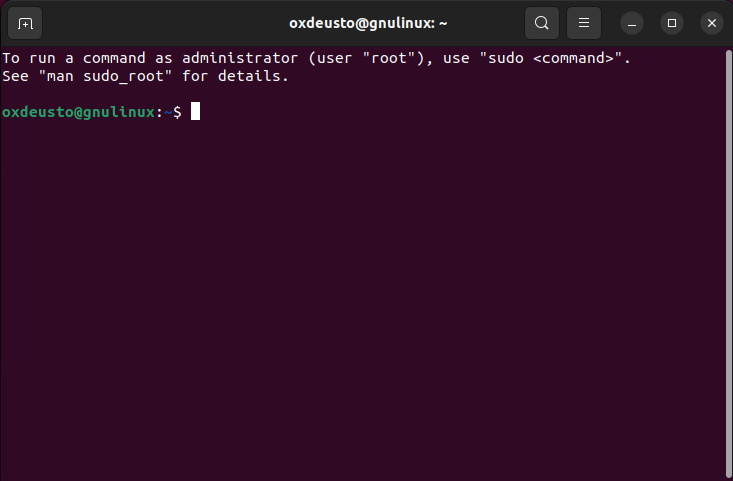
\includegraphics[width=0.80\linewidth]{resources/images/terminal_abrir.png}
    \caption{Aspecto de la terminal al abrirla}
\end{figure}

Vamos a fijarnos en el texto:

\begin{tcolorbox-code}
\begin{lstlisting}
oxdecode@gnulinux:~$
\end{lstlisting}
\end{tcolorbox-code}

A este texto se le llama shell prompt. ¿Pero qué significa? Vamos a verlo por partes:

\begin{itemize}
    \item Nuestro nombre de usuario se encuentra a la izquierda del carácter @ (que hace de separador). En este caso es "oxdecode".
    \item Después del @ está nuestro hostname (el nombre de nuestro ordenador), también configurado por nosotros al instalar el sistema. En este caso es "gnulinux".
    \item El carácter \~{} es un carácter especial. Siempre que lo veas en el shell prompt significa que te encuentras en tu directorio de usuario en /home. En este caso, la dirección absoluta sería /home/oxdecode Además, es la dirección por defecto en que se abre la terminal. Si en el directorio de usuario hubiera otro directorio llamado "fotos", y se abriera la terminal ahí, el shell prompt sería así:

    \begin{tcolorbox-code}
\begin{lstlisting}
    oxdecode@gnulinux:~/fotos$
\end{lstlisting}
\end{tcolorbox-code}

    \item El carácter del dólar (\$) al final del prompt no es más que un indicador que muestra que puedes escribir comandos a nivel de usuario. Si en vez de salir un \$ saldría un \#, significa que tienes permisos de root.
\end{itemize}

\section{Direcciones}
Ahora que has visto direcciones en el shell prompt, es hora de hablar sobre cómo funcionan. Como se mencionó en el Tema 2, la forma en la que se ordenan los ficheros en un sistema operativo de Linux es jerárquica. Todos los directorios y ficheros parten de un solo sitio, root. Esta es su dirección:

\begin{tcolorbox-code}
\begin{lstlisting}
/
\end{lstlisting}
\end{tcolorbox-code}

En root se encuentran todos los directorios del SO, como /home, /etc, /tmp... El directorio de nuestro usuario se encuentra en /home, donde están todos los directorios de usuarios. Si tu nombre de usuario es "oxdecode", la dirección del directorio será la siguiente:

\begin{tcolorbox-code}
\begin{lstlisting}
/home/oxdecode/
\end{lstlisting}
\end{tcolorbox-code}

El direccionamiento es la forma que tenemos de localizar archivos, ya sea para referenciarlos en un programa o para abrirlos nosotros mismos. Hay dos tipos de direccionamiento:

\begin{itemize}
    \item \textbf{Direccionamiento absoluto}: Cuando referencias la dirección del fichero desde root (/). La ventaja de utilizar el direccionamiento absoluto es que la dirección va a ser válida independientemente del directorio en el que te encuentres, porque inicias el direccionamiento desde root. Un ejemplo de direccionamiento absoluto es precisamente el ejemplo de dirección previo:
    \begin{tcolorbox-code}
\begin{lstlisting}
/home/oxdecode/
\end{lstlisting}
\end{tcolorbox-code}
    \item \textbf{Direccionamiento relativo}: Cuando referencias la dirección del fichero desde el directorio en el que estás trabajando. La ventaja de este tipo de direccionamiento es que puede ser muy útil en programas de código. Si quieres programar una aplicación que necesite referenciar un archivo en el mismo directorio en el que se ejecuta la aplicación, es más conveniente utilizar direccionamiento relativo, ya que tú, como programador/a, no tienes por qué conocer la estructura de archivos de un ordenador que no es tuyo. Fíjate en esta estructura de archivos:
\end{itemize}

\begin{figure}[H]
    \centering
    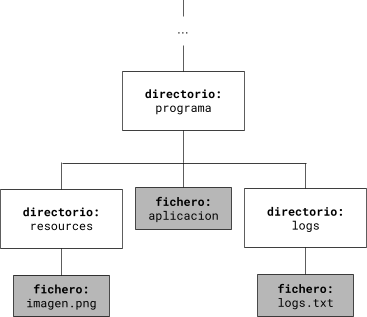
\includegraphics[width=0.80\linewidth]{resources/images/estructura-archivos-1.png}
    \caption{Estructura de archivos de ejemplo}
\end{figure}

Tenemos un directorio llamado "programa", con otros dos directorios dentro, "resources" y "logs". Los tres puntos indican que no sabemos dónde está almacenado "programa", pero no nos importa porque podemos utilizar el direccionamiento relativo para referenciar los ficheros que sí sabemos dónde están, "imagen.png" (en programa/resources), "logs.txt" (en programa/logs) y "aplicación" (que es un fichero ejecutable en programa).

Pongamos que el programa aplicación necesita utilizar el fichero "imagen.png". Para ello, podemos poner en el código la ruta relativa de la imagen. Como el fichero está en programa, la ruta relativa de la imagen es esta:

\begin{tcolorbox-code}
\begin{lstlisting}
resources/imagen.png\begin{figure}
\end{lstlisting}
\end{tcolorbox-code}

Pon atención a que no escribimos una barra al principio de la dirección, porque de escribirla estaríamos accediendo al fichero desde root, de forma absoluta, algo indeseado para este ejemplo, ya que no encontraría el fichero. Como resources está directamente dentro de "programa", podemos referenciarlo directamente, sin poner nada previamente. Es por esto que el direccionamiento relativo es tan útil.

Vamos ahora con un ejemplo un poco más raro: por lo que sea, ahora el programa se encuentra en la carpeta programa/resources, y queremos acceder a logs.txt. La estructura de archivos es esta:

\begin{figure}[H]
    \centering
    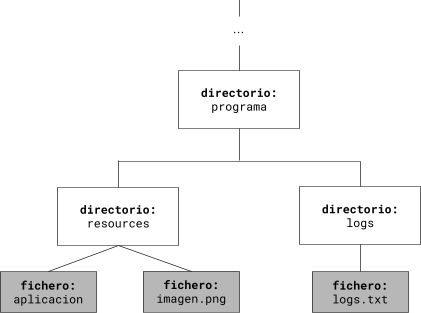
\includegraphics[width=0.80\linewidth]{resources/images/estructura_ficheros_2.png}
    \caption{Otra estructura de archivos.}
\end{figure}

Aquí acceder a logs.txt es un poco más complicado, porque tenemos que ir hacia atrás para acceder al directorio de programa/logs. La forma de acceder a logs.txt desde resources sería la siguiente:

\begin{tcolorbox-code}
\begin{lstlisting}
../logs/logs.txt
\end{lstlisting}
\end{tcolorbox-code}

Al incluir dos puntos en la dirección estamos representando que queremos dar "un paso para atrás" en la jerarquía de directorios. Al usarlos, en este caso nos iríamos al directorio "programa", donde podemos acceder a logs y posteriormente a logs.txt.

Cabe destacar que el direccionamiento relativo no solo se usa en código de programas, lo podemos utilizar también en comandos de terminal, si así lo necesitamos. Veremos cómo en el siguiente apartado.

\section{Navegando entre directorios}
Como hemos aprendido en el apartado anterior, las direcciones son esenciales para trabajar en la terminal. Hemos visto también cómo la terminal puede estar en una dirección u otra, y cómo afecta eso a nuestras tareas. Una de las cosas que más se suele hacer es desplazarse alrededor de tu sistema de archivos. Para ello se utiliza el comando cd.

cd (o change directory) es un comando que, como su propio nombre indica, nos permite movernos entre directorios. El uso es muy simple:

\begin{tcolorbox-code}
\begin{lstlisting}
$ cd <dirección del directorio>
\end{lstlisting}
\end{tcolorbox-code}

Como ejemplo vamos a imaginarnos que estamos en el directorio /var y que queremos movernos al directorio de nuestro usuario. Una forma de hacerlo sería la siguiente.

\begin{tcolorbox-code}
\begin{lstlisting}
$ cd /home/oxdecode
\end{lstlisting}
\end{tcolorbox-code}

En este caso estamos utilizando la dirección absoluta de nuestro directorio para movernos a él. Sin embargo, hay otra forma más rápida de acceder a este directorio. Como hemos mencionado anteriormente, el carácter ~ se suele asociar con nuestro directorio de usuario. Observa:

\begin{tcolorbox-code}
\begin{lstlisting}
$ cd ~
\end{lstlisting}
\end{tcolorbox-code}

Este comando es otra forma igual de válida que la otra para acceder a tu directorio de usuario. De hecho, los dos comandos son equivalentes. Además, puedes usar el mismo carácter para acceder a otros directorios en el directorio de usuario. Considerando que creamos el directorio "fotos" dentro del directorio y que seguimos en /var (aunque este ejemplo funciona en cualquier directorio ya que es direccionamiento absoluto)...

\begin{tcolorbox-code}
\begin{lstlisting}
$ cd ~/fotos 
\end{lstlisting}
\end{tcolorbox-code}

Este comando nos movería a "fotos". Y ya para terminar, podemos volver a nuestro directorio de usuario de forma relativa.

\begin{tcolorbox-code}
\begin{lstlisting}
$ cd ..
\end{lstlisting}
\end{tcolorbox-code}

Ten en cuenta que el doble punto se puede usar más de una vez para moverse más hacia atrás. Desde ~, poniendo el doble punto dos veces, llegaríamos a root (el primer doble punto nos llevaría a /home y el segundo a /):

\begin{tcolorbox-code}
\begin{lstlisting}
$ ../..
\end{lstlisting}
\end{tcolorbox-code}

Cabe mencionar la existencia del comando pwd (Print Working Directory), un comando que nos imprime la dirección absoluta del directorio en el que nos encontramos. Si me encuentro en ~/fotos y ejecuto el comando nos devolvería esto:

\begin{tcolorbox-code}
\begin{lstlisting}
$ pwd
/home/oxdecode/fotos
\end{lstlisting}
\end{tcolorbox-code}

Con toda esta información, ya sabemos lo básico sobre la terminal y cómo navegar en ella. Es momento de aprender todo lo demás. En el próximo tema empezaremos con bash, aprendiendo unos comandos variados que nos ayudarán a adaptarnos poco a poco a usar la terminal de forma cotidiana.

\chapter{Bash}

Como ya hemos comentado, bash es un shell, es decir, un intérprete de comandos. Es el programa con el que nos comunicamos para realizar tareas en la terminal. Fue creado por GNU y es sin duda el shell más utilizado en sistemas operativos Linux, aunque no el único. En este tema vamos a aprender a utilizar los comandos fundamentales de bash, que nos van a dar un conocimiento sobre la terminal que nos permitirá usarla de una forma cotidiana.

\section{Saber documentarse}
A medida que usamos la terminal, aprenderemos a usar muchos comandos. Sin embargo, es posible que con el tiempo se nos olvide el funcionamiento de alguno de ellos o las opciones y argumentos que utiliza. Esto es común, por lo tanto tenemos que saber cómo documentarnos sobre los comandos. También es importante saber los recursos que nos otorga el sistema operativo para trabajar en la terminal. Por eso, el primer comando que vamos a aprender es man.

\begin{command-info}
{man}
{Es el manual de referencia del sistema.}
{man <comando>}
{Ninguna}
{man man o man -?}
\end{command-info}

man (MANual) guarda detalladamente las instrucciones de cada parámetro y opción que ofrece el comando que estamos consultando. Por ejemplo, veamos el manual del comando pwd.

\begin{tcolorbox-code}
\begin{lstlisting}
$ man pwd
\end{lstlisting}
\end{tcolorbox-code}

Al ejecutar este comando, se nos abrirá una interfaz:
\begin{figure}[H]
    \centering
    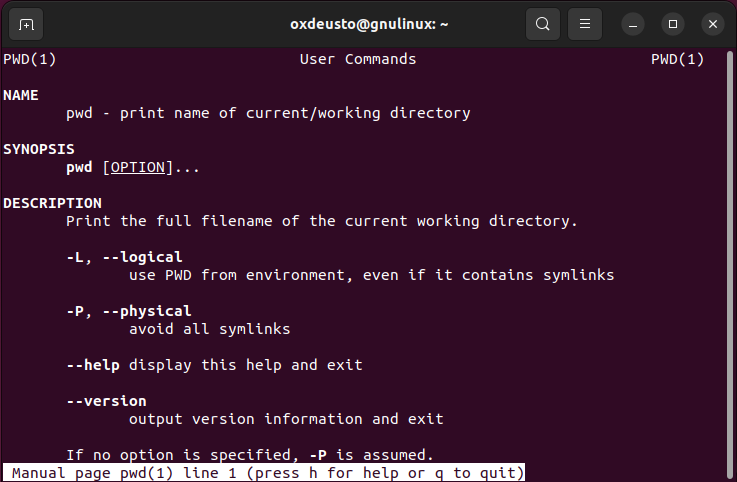
\includegraphics[width=0.80\linewidth]{resources/images/man.png}
    \caption{Manual de referencia del comando pwd.}
\end{figure}

man es muy útil porque nos permite consultar información de cada comando sin salir de la terminal, sin la necesidad tampoco de tener conexión a internet. Al abrir un manual, puede salir de él presionando la tecla q de (quit)

Es importante destacar que algunos pocos comandos no tienen una entrada en man, pero esto no es un problema, ya que ofrecen una opción de ayuda. Ésta normalmente es -h o --help.

Si bien man es una forma rápida de saber el uso general de un comando y la funcionalidad detallada de sus argumentos y opciones, las entradas del manual no suelen incluir ejemplos. Es por eso que, si deseas explicaciones más prácticas consultes internet. Foros de informática como StackOverflow (https://stackoverflow.com/) tienen respuestas a cualquier duda que se te pueda ocurrir. El foro de AskUbuntu (https://askubuntu.com/) tiene preguntas más relacionadas con Ubuntu, pero también es un buen lugar donde resolver dudas.

\section{Manipulando nuestro entorno de fichero}
Para sorpresa de nadie, una de las funcionalidades más importantes de un sistema operativo es poder crear, modificar y eliminar ficheros. El shell de bash, naturalmente, nos ofrece comandos para poder realizar estas tareas básicas. Vamos a mirarlas una a una:

\begin{command-info}
{mkdir}
{Crear directorios.}
{mkdir <dirección del directorio>}
{-p}
{man mkdir o mkdir --help}
\end{command-info}

mkdir (o MaKe DIRectory) nos permite crear directorios. Veamos un ejemplo. Si quiero crear un directorio llamado "documentos" en el directorio en el que me encuentro, podríamos usar mkdir con direccionamiento relativo:

\begin{tcolorbox-code}
\begin{lstlisting}
$ mkdir documentos
\end{lstlisting}
\end{tcolorbox-code}

Esto crea un directorio llamado "documentos" dentro del directorio en el que me encuentro. Recuerda que se puede conseguir el mismo resultado con direccionamiento absoluto. Si quiero crear el directorio en mi carpeta de usuario, puedo hacer...

\begin{tcolorbox-code}
\begin{lstlisting}
$ mkdir /home/oxdecode/documentos
\end{lstlisting}
\end{tcolorbox-code}

o...

\begin{tcolorbox-code}
\begin{lstlisting}
$ mkdir ~/documentos
\end{lstlisting}
\end{tcolorbox-code}

Si queremos crear más de un directorio a la vez, cada uno dentro de otro, tenemos que usar la opción -p. Observa:

\begin{tcolorbox-code}
\begin{lstlisting}
$ mkdir -p documentos/2024/mayo
\end{lstlisting}
\end{tcolorbox-code}

Este comando sería equivalente a hacer la siguiente sucesión de comandos:

\begin{tcolorbox-code}
\begin{lstlisting}
$ mkdir documentos
$ mkdir documentos/2024
$ mkdir documentos/2024/mayo
\end{lstlisting}
\end{tcolorbox-code}

Hemos aprendido a crear directorios, vamos a aprender ahora cómo crear ficheros:

\begin{command-info}
{touch}
{Crear ficheros (archivos).}
{touch <dirección del fichero>}
{Ninguna}
{man touch o touch --help}
\end{command-info}

El comando touch te permite crear ficheros en una dirección específica. El uso es el siguiente:

\begin{tcolorbox-code}
\begin{lstlisting}
$ touch documentos/2024/mayo/factura.txt
\end{lstlisting}
\end{tcolorbox-code}

Este fichero crea en ~/documentos/2024/mayo un fichero llamado "factura" de extensión .txt.

Hemos aprendido a crear directorios y ficheros. Más tarde aprenderemos a manejar los permisos de los ficheros, pero por ahora, veamos cómo eliminar ficheros o directorios.

\begin{center}
  \rule{15cm}{0.4pt}
\end{center}
\textbf{rm}\\
Utilidad: Elimina directorios o ficheros.\\
Forma de uso general: rm <dirección del directorio o fichero>\\
Opciones comunes: -r, -d\\
Ayuda: man rm o rm --help
\begin{center}
  \rule{15cm}{0.4pt}
\end{center}

\begin{command-info}
{rm}
{Elimina directorios o ficheros.}
{rm <dirección del directorio o fichero>}
{-r, -d}
{man rm o rm --help}
\end{command-info}

rm (ReMove) es el comando que utilizamos para eliminar directorios o ficheros. Para eliminar ficheros, nos basta con hacer lo siguiente:

\begin{tcolorbox-code}
\begin{lstlisting}
$ rm ~/documentos/2024/mayo/factura.txt
\end{lstlisting}
\end{tcolorbox-code}

Esto eliminará el fichero "factura.txt". Una vez más, recuerda que también se puede utilizar direccionamiento relativo para todas estas tareas. Para eliminar directorios, no nos basta con seguir la misma estructura:

\begin{tcolorbox-code}
\begin{lstlisting}
$ rm ~/documentos/2024/mayo/
rm: cannot remove ‘documentos/2024/mayo’: is a directory
\end{lstlisting}
\end{tcolorbox-code}

rm requiere la opción -r o -d para eliminar directorios. Si queremos eliminar un directorio de forma recursiva, tenga ficheros dentro o no, utilizamos -r (recursive).

\begin{tcolorbox-code}
\begin{lstlisting}
$ rm -r ~/documentos
\end{lstlisting}
\end{tcolorbox-code}

Esto va a eliminar "documentos" y todo lo que había en su interior.

Existe también la opción -d, que elimina sólo directorios vacíos. Es una opción más segura de utilizar el comando rm.

\textbf{\textbf{Nota:}} Existe el comando rmdir, que elimina directorios siempre que estén vacíos, como el comando rm -d.
Ya sabemos crear y eliminar directorios y ficheros. Antes de ver cómo copiarlos o moverlos, vamos a aprender a usar un comando muy útil, que si bien no modifica nuestro entorno de trabajo, es una herramienta muy importante.

\begin{command-info}
{ls}
{Enlista el contenido de un directorio}
{ls <dirección>}
{-R, -a, -l...}
{man ls o ls --help}
\end{command-info}

ls (LiSt) es un comando que nos permite ver el contenido de un directorio, tanto sus ficheros como otros directorios dentro. Para mostrarlo, vamos a movernos a root y listar el contenido:

\begin{tcolorbox-code}
\begin{lstlisting}
$ cd /
$ ls
\end{lstlisting}
\end{tcolorbox-code}

Obtendremos esto:
\begin{figure}[H]
    \centering
    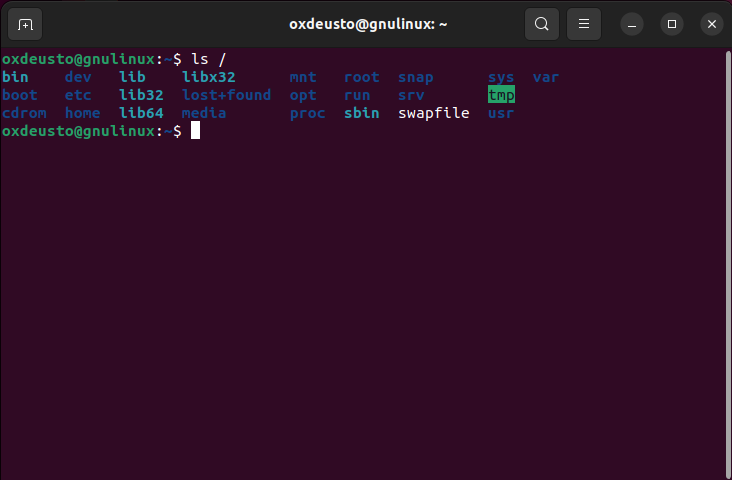
\includegraphics[width=0.8\linewidth]{resources/images/ls_1.png}
    \caption{Comando ls.}
\end{figure}

La mayoría de los elementos (los que están en azul oscuro) son directorios, de los cuales se pueden ver algunos que ya conocemos por el Tema 1, como /bin, /etc /home... Esto es root (/), y todos los datos del sistema operativo los puedes encontrar aquí, en alguno de estos directorios.

ls es un comando con bastantes opciones, y es recomendable consultar su manual ya que hay opciones de mucha utilidad. Vamos a consultar algunas de las más importantes.

Con la opción -R podemos listar recursivamente cada directorio dentro del directorio que estamos enlistando. Es decir, que además de listar el contenido del directorio deseado, lista también el contenido de los directorios dentro de éste. Como listar recursivamente / implicaría tener que listar literalmente nuestro sistema operativo entero, sería conveniente probarlo en un directorio menos denso, como podría ser nuestra carpeta "documentos":

\begin{tcolorbox-code}
\begin{lstlisting}
$ ls -R ~/documentos
\end{lstlisting}
\end{tcolorbox-code}
\begin{figure}[H]
    \centering
    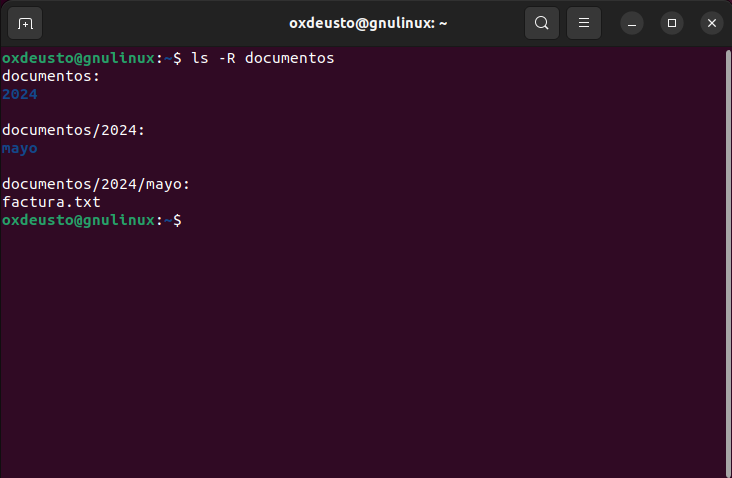
\includegraphics[width=0.80\linewidth]{resources/images/ls_2.png}
    \caption{ls recursivo.}
\end{figure}

Al usar la opción -R podemos ver el contenido de cada subdirectorio en documentos.

Con la opción -a podemos listar los ficheros ocultos del directorio. Un fichero oculto es un fichero que tiene como primer carácter en el nombre un punto. Para realizar la prueba, vamos a crear un fichero oculto en ~:

\begin{tcolorbox-code}
\begin{lstlisting}
$ touch ~/.secreto.txt
$ ls ~
\end{lstlisting}
\end{tcolorbox-code}

Al listar el directorio, verás como el fichero recién creado no se muestra.

\begin{figure}[H]
    \centering
    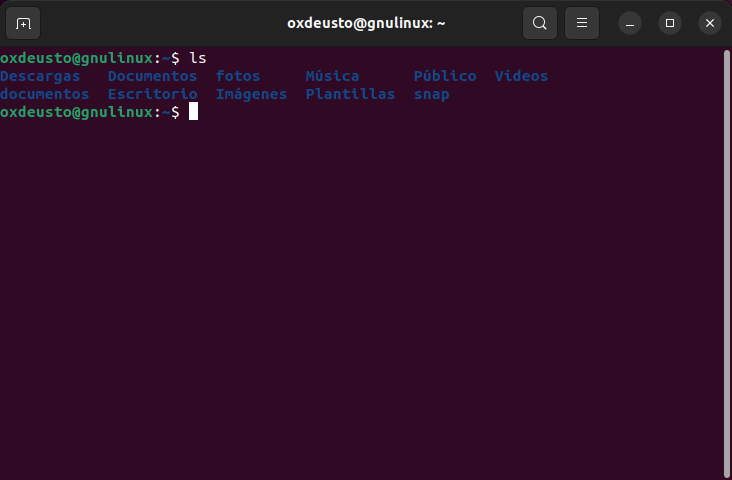
\includegraphics[width=0.80\linewidth]{resources/images/ls_3.png}
    \caption{ls normal, no se muestran ficheros ocultos.}
\end{figure}

Esto se debe a que ls no imprime ficheros ocultos a no ser que utilicemos la opción -a:
\begin{tcolorbox-code}
\begin{lstlisting}
$ ls -a ~
\end{lstlisting}
\end{tcolorbox-code}

\begin{figure}[H]
    \centering
    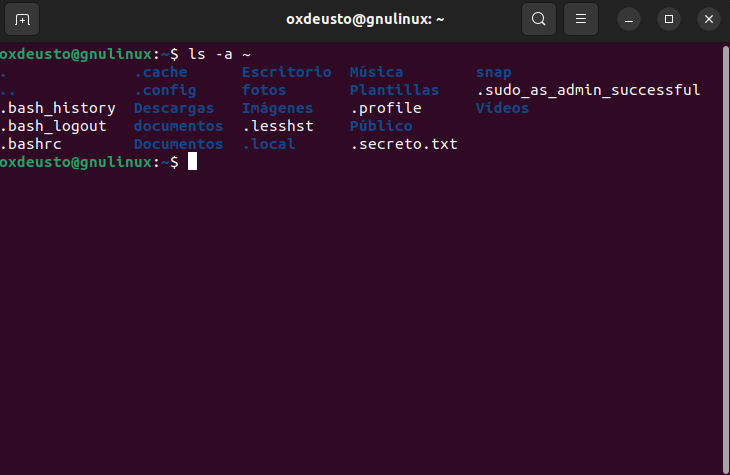
\includegraphics[width=0.80\linewidth]{resources/images/ls_4.png}
    \caption{ls -a, nos muestra también los ficheros ocultos.}
\end{figure}

Fíjate cómo además de .secreto.txt, \~ contiene otros ficheros ocultos que no hemos creado nosotros. Estos ficheros tienen diferentes utilidades, por ejemplo .bash\_history es un log de los comandos que hemos utilizado en la terminal. .bashrc es un script que se ejecuta cuando iniciamos sesión. .bash\_logout se ejecuta cuando se cierra una shell. Para nuestro contexto, estos ficheros no nos interesan, pero pueden ser muy útiles en algunas situaciones.

Cabe destacar que es posible utilizar más de una opción en un comando, obteniendo así la funcionalidad de ambas opciones:

\begin{tcolorbox-code}
\begin{lstlisting}
$ ls -aR # ls -a -R tambíen sirve
\end{lstlisting}
\end{tcolorbox-code}

Además de crear y eliminar directorios y ficheros, nos puede ser de utilidad copiarlos y moverlos, además de renombrarlos:

\begin{command-info}
{cp}
{Copia un fichero o directorio a una dirección.}
{cp <dir. origen> <dir. destino>}
{-r}
{man cp o cp --help}
\end{command-info}

cp (CoPy) es un comando que nos permite copiar un fichero o un directorio. Como esta operación implica dos direcciones, el formato que utiliza es uno diferente al que hemos visto hasta ahora. Vamos a copiar el fichero factura.txt a nuestra carpeta de usuario, estando en esa misma carpeta:

\begin{tcolorbox-code}
\begin{lstlisting}
$ cp documentos/2024/mayo/factura.txt .
\end{lstlisting}
\end{tcolorbox-code}

Fíjate cómo en la dirección de destino colocamos nada más que un punto. Este punto representa un "aquí". Cuando colocamos un punto en la dirección de destino estamos indicando que queremos copiar el fichero en el directorio en el que nos encontramos, en este caso en ~.

Para copiar directorios hay que usar una opción, -r.

\begin{tcolorbox-code}
\begin{lstlisting}
$ cp -r documentos .
\end{lstlisting}
\end{tcolorbox-code}

\begin{command-info}
{mv}
{Mueve un directorio o fichero a otra dirección.}
{mv <dir. origen> <dir. destino>}
{Ninguna}
{man mv o mv --help}
\end{command-info}

mv (MoVe) sigue la misma estructura que cp, pero en vez de copiar el fichero o el directorio, cambia su dirección. Esto tiene una funcionalidad extra muy importante. Cambiar nombres. Al fin y al cabo, si cambias la dirección de un fichero o directorio, tienes la posibilidad de cambiar su nombre también.

\begin{tcolorbox-code}
\begin{lstlisting}
$ mv documentos/2024/mayo/factura.txt ./factura\_mayo\_2024.txt
\end{lstlisting}
\end{tcolorbox-code}

En este caso estoy moviendo factura.txt al directorio en el que estoy (~), dándole el nombre de "factura\_mayo\_2024.txt". No hace falta cambiar el directorio del fichero para cambiar su nombre:

\begin{tcolorbox-code}
\begin{lstlisting}
$ cd documentos/2024/mayo
$ mv factura.txt factura_mayo_2024.txt
\end{lstlisting}
\end{tcolorbox-code}

Gracias a todo estos comandos (mkdir, touch, rm, ls, cp y mv) ya sabemos cómo modificar nuestro entorno de archivos. En el próximo apartado nos vamos a centrar en la modificación de ficheros. Está bien ser capaz de crear y eliminar ficheros, pero si no sabemos cómo modificar su contenido, no nos pueden ser de mucha utilidad.

\section{Editar ficheros}
Editar ficheros es una funcionalidad clave en cualquier sistema operativo. Gracias a ésta podemos sacarle provecho a los ficheros, para almacenar información o incluso programar en ellos. Para esto utilizamos los editores de texto (IDE). Uno muy conocido y utilizado por muchos programadores y programadoras es Visual Studio Code, que te ofrece incontables herramientas para optimizar tu programación. VS Code, al igual que muchos otros IDEs como Eclipse, NetBeans o IntelliJ, contiene interfaces gráficas que facilitan su uso para el usuario promedio, pero también existen editores de texto para terminales.



Uno de los más utilizados gracias a lo extremadamente personalizable que es, es vim (o neovim). Este IDE ha ganado fama entre los programadores/as que pasan la mayor parte de su tiempo en la terminal. Puede convertirse en un entorno de programación muy rápido, superando en eficiencia incluso a los IDEs con interfaces gráficas. Sin embargo, aprender a utilizarlo no es un proceso fácil. Por ello, vamos a fijarnos en un editor de texto que suele venir por defecto en muchas distribuciones, que es perteneciente al proyecto GNU: nano.

\begin{command-info}
{nano}
{Abre el editor de texto "nano".}
{nano <fichero a editar (opcional)>}
{Ninguna}
{man nano o nano --help}
\end{command-info}

nano es un editor de texto básico, que en la práctica no es del todo recomendable usarlo, y menos para programar. Pero para este curso nos sirve como ejemplo de editor de texto. Para abrirlo basta con escribir...

\begin{tcolorbox-code}
\begin{lstlisting}
$ nano
\end{lstlisting}
\end{tcolorbox-code}

...pero se suele especificar una dirección a un fichero, exista o no, para guardarlo directamente al terminar sin tener que especificar su nombre dentro del editor.

Independientemente de si especifiquemos una dirección o no, se nos abrirá una interfaz como esta:

\begin{figure}[H]
    \centering
    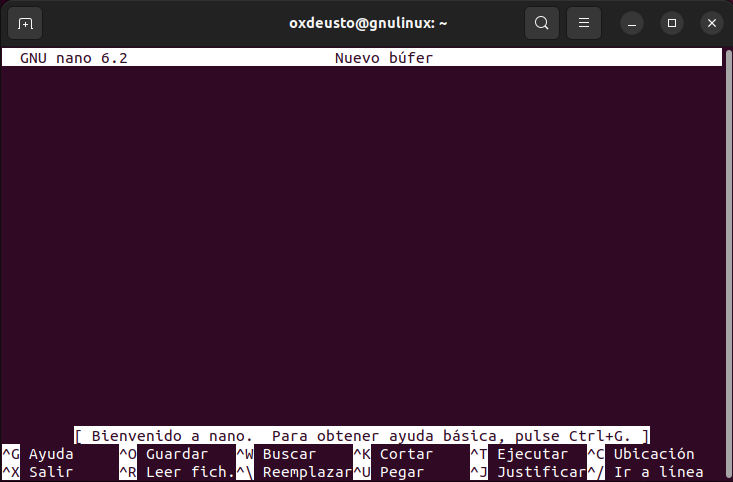
\includegraphics[width=0.80\linewidth]{resources/images/nano.png}
    \caption{Vista de nano.}
\end{figure}

En esta interfaz ya podemos escribir en el fichero como si fuera un editor de texto normal y corriente. En la parte inferior de la interfaz vemos unas cuantas opciones. Cada instrucción tiene el carácter "\^" acompañado de una letra. Ese carácter representa la tecla ctrl, es decir, que si queremos guardar el fichero tenemos que pulsar la combinación de teclas ctrl + o.

Como se puede observar, este editor de texto es muy sencillo de usar, así que tampoco hace falta que le dediquemos mucho tiempo a ver sus funcionalidades.

Para futuros ejemplos, vamos a escribir algo en este fichero y lo vamos a guardar en la dirección del fichero de facturas.txt. De esta manera, vamos a sobreescribirlo con el texto que hemos escrito con nano:

\begin{figure}[H]
    \centering
    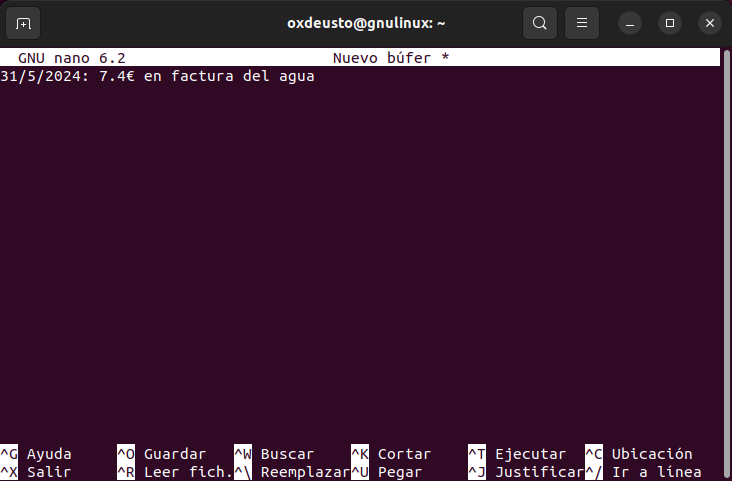
\includegraphics[width=0.80\linewidth]{resources/images/nano_2.png}
    \caption{Texto escrito en nano.}
\end{figure}

Le damos a ctrl + o y escribimos la dirección.

\begin{figure}[H]
    \centering
    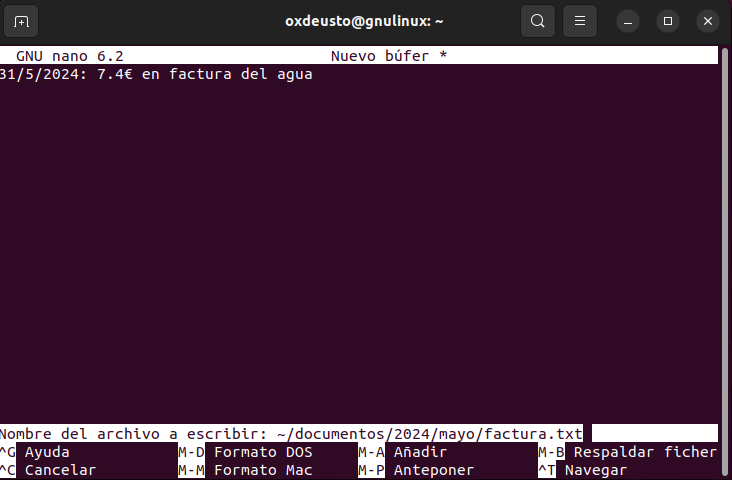
\includegraphics[width=0.75\linewidth]{resources/images/nano_3.png}
    \caption{Entrada de dirección del fichero.}
\end{figure}

\textbf{Nota:} En apartados anteriores hubo un ejemplo en el que movimos este fichero a ~, así que si estás ejecutando los comandos de estos apuntes en tu máquina, tendrás dos facturas, una en ~ y otra en ~/documentos/2024/mayo/, y en este ejemplo no estarás sobreescribiendo el fichero, lo estarías creando de nuevo en el directorio "mayo". Sin embargo, el resultado no cambia.

Ahora que hemos aprendido a escribir archivos, vamos a aprender a leerlos sin usar un editor de texto:

\begin{command-info}
{cat}
{Imprime los ficheros que recibe como parámetro.}
{cat <dir. fichero> <dir. fichero2>}
{Ninguna}
{man cat o cat --help}
\end{command-info}

cat (conCATenate) concatena (une) el contenido de los ficheros que recibe como parámetros y los imprime. Si bien puedes consultar el contenido de un fichero mediante un editor de texto, cat es el comando que se usa para imprimir un fichero en consola, porque nos puede permitir usar el contenido de un fichero como datos de entrada para algún comando mediante el uso de los pipes (más sobre esto más tarde). El uso es muy sencillo, vamos a imprimir el fichero que acabamos de crear:

\begin{tcolorbox-code}
\begin{lstlisting}
$ cat ~/documentos/2024/mayo/factura.txt
31/5/2024: 7.4 € en factura del agua
\end{lstlisting}
\end{tcolorbox-code}

Si creo otro fichero llamado factura2.txt con el texto "31/5/2024: 78.34 € en factura de la luz" y lo añado como argumento junto con factura.txt, el resultado es de esperar:

\begin{tcolorbox-code}
\begin{lstlisting}
$ cat factura.txt factura2.txt # Estando en el directorio mayo/
31/5/2024: 7.4 € en factura del agua
31/5/2024: 78.34 € en factura de la luz
\end{lstlisting}
\end{tcolorbox-code}

\section{Usuarios}
GNU/Linux, al igual que los demás sistemas operativos principales del mercado, ofrece un sistema de usuarios. Sin embargo, Linux da un paso más en cuanto al control sobre éstos, ofreciéndonos más utilidades sobre los permisos de cada usuario.

En Linux hay tres tipos de usuarios:

\begin{itemize}
    \item \textbf{Usuario root}: Es el usuario con permisos absolutos sobre el sistema. Además de esto, se distingue de los demás usuarios por tener el UID (User ID) 0. En nuestros usuarios personales, cuando queremos realizar una tarea que requiere permisos especiales (de nivel root), utilizamos el comando sudo <comando> para heredar permisos de root para ese comando, una vez proporcionada la contraseña de root.

    \item \textbf{Usuarios personales}: Son los usuarios que creamos nosotros. En la mayoría de los casos tienen sus directorios propios en /home y sus UIDs parten del número 1000. En función de nuestras configuraciones, cada usuario tiene permisos diferentes ante diferentes ficheros.

    \item \textbf{Usuarios del sistema}: Son usuarios que crea el propio sistema operativo o programas que tengamos instalados, y pueden tener muchos usos diferentes dependiendo de su origen. Sus UIDs son menores de 1000 y normalmente tienen permisos de sudo, pero este no es siempre el caso. Para este curso este tipo de usuario no nos interesa, pero sé consciente de que estos usuarios existen y tienen un papel importante en el funcionamiento de muchos programas.
\end{itemize}

Ahora vamos a ver cómo crear un usuario personal en Linux:

\begin{command-info}
{useradd}
{Permite crear usuarios.}
{sudo useradd <nombre de usuario>}
{-m}
{man useradd o useradd --help}
\end{command-info}

useradd fundamentalmente nos permite crear usuarios, pero vamos a necesitar otros comandos si queremos configurar un usuario por completo. En cualquier caso, creamos un usuario de la siguiente manera:

\begin{tcolorbox-code}
\begin{lstlisting}
$ sudo useradd -m franz
\end{lstlisting}
\end{tcolorbox-code}

Con este comando creamos un usuario llamado "franz". Nótese cómo usamos sudo para este comando. Crear usuarios requiere permisos de root, por lo cual necesitaremos introducir de nuevo nuestra contraseña, y que formemos parte del grupo de sudoers (lo veremos más adelante). 

También usamos la opción -m. Esta opción, además de crear el usuario, crea un directorio de usuario para él, en /home. Ahora vamos a darle una contraseña a este usuario:

\begin{command-info}
{passwd}
{Crea o modifica contraseñas de usuarios.}
{sudo passwd}
{-d}
{man passwd o passwd}
\end{command-info}

\begin{tcolorbox-code}
\begin{lstlisting}
$ sudo passwd franz
\end{lstlisting}
\end{tcolorbox-code}

Este comando te pedirá una contraseña y que la repitas, para asignarla a Franz. Se puede eliminar la contraseña del usuario utilizando la opción -d (delete).

Con estos dos comandos básicos podemos crear un usuario y establecer su contraseña. Ahora vamos a aprender a configurar otras características de usuarios:

\begin{command-info}
{usermod}
{Permite modificar características de usuarios.}
{sudo usermod [opción(es)] <usuario>}
{-aG, -l...}
{man usermod o usermod --help}
\end{command-info}

usermod tiene varios usos. Uno de los más importantes es poder cambiar el grupo al que pertenece el usuario. Los grupos los veremos en detalle en el próximo apartado, pero por ahora, hay un grupo en concreto que permite a sus usuarios poder usar el comando sudo. Para darle a Franz permisos de sudo, podemos usar el siguiente comando:

\begin{tcolorbox-code}
\begin{lstlisting}
$ sudo usermod -aG sudo franz
\end{lstlisting}
\end{tcolorbox-code}

La opción -G nos indica que queremos meter a Franz en los grupos que le indicamos (separado por comas). En este caso, queremos añadirle al grupo de sudo (sudoers). Los usuarios dentro de este grupo tienen acceso al comando sudo. Añadimos la opción -a (append) para añadirle a Franz al grupo sudo sin que se salga de los demás grupos en los que está. De no incluir -a, Franz se añadiría a sudo pero abandonaría sus otros grupos.

usermod tiene muchos otros usos, estos son algunos más:

\begin{tcolorbox-code}
\begin{lstlisting}
$ sudo usermod -u 1024 franz # Cambia el UID de franz a 1024
$ sudo usermod -l nuevo_nombre franz # Cambia el nombre de franz
$ sudo usermod -L franz # Deshabilita la cuenta de franz
$ sudo usermod -U franz # Rehabilita la cuenta de franz
\end{lstlisting}
\end{tcolorbox-code}

Existen bastantes usos más para este comando, así que es recomendable consultar la página del manual de usermod para más información.

Ahora que hemos aprendido a cambiar de usuarios, vamos a ver cómo cambiar de usuario en la terminal:

\begin{command-info}
{su}
{Permite cambiar de usuario.}
{su <usuario al que quieres cambiar>}
{Ninguna}
{man usermod o usermod --help}
\end{command-info}

su (Switch User) nos abre una shell dentro de nuestra terminal que nos permite ejecutar comandos bajo otro usuario, una vez escribes su contraseña.

\begin{tcolorbox-code}
\begin{lstlisting}
$ su franz
$ # Shell nueva bajo el usuario franz
\end{lstlisting}
\end{tcolorbox-code}

Una forma de comprobar que hemos cambiado de usuario correctamente es mediante el comando whoami:

\begin{command-info}
{whoami}
{Imprime el nombre de usuario de tu shell actual}
{whoami}
{Ninguna}
{man whoami o whoami --help}
\end{command-info}

\begin{tcolorbox-code}
\begin{lstlisting}
$ whoami
franz
$
\end{lstlisting}
\end{tcolorbox-code}

Hemos ejecutado whoami bajo el usuario franz, por ello nos devuelve "franz" y no "oxdecode". Ahora sabemos que hemos cambiado de usuario correctamente.

Si queremos volver a nuestro usuario original, basta con escribir "exit", o pulsando la combinación de teclas ctrl + D. Veremos cómo nuestro shell prompt vuelve a aparecer.

Para terminar vamos a ver cómo eliminar un usuario:

\begin{command-info}
{userdel}
{Elimina un usuario.}
{sudo userdel <usuario>}
{-r, -f}
{man userdel o userdel --help}
\end{command-info}

Si queremos eliminar un usuario, normalmente se hace de esta manera:

\begin{tcolorbox-code}
\begin{lstlisting}
$ sudo userdel -r franz
\end{lstlisting}
\end{tcolorbox-code}

La opción -r, además de eliminar el usuario, elimina también su carpeta de usuario. De no incluir esta opción, los ficheros en el directorio se quedarían sin propietario.

\section{Grupos}

A diferencia de Windows, los usuarios de Linux pueden formar parte de unos conjuntos llamados grupos. Los grupos nos facilitan la gestión de usuarios.

Un ejemplo para el uso de grupos podría ser en una empresa. Imagínate que en un sistema de una empresa trabajan dos tipos de trabajadores: administradores/as y técnicos/as. Tendría sentido que los administradores/as tengan acceso a ficheros más privados de la empresa, o que puedan ejecutar programas que los técnicos/as no. Para esto podemos crear grupos, ya que con ellos podemos establecer un sistema de permisos generalizado para cada grupo.

Uno de los grupos que viene por defecto en nuestro sistema es el grupo sudo (a veces llamado "wheel"), que contiene en él todos los usuarios con permisos para ejecutar comandos con sudo. Por eso, cuando queremos hacer que un usuario tenga acceso al comando sudo, basta con añadirle a este grupo.

Además de esto, los grupos tienen otro concepto importante que tiene que ver con los usuarios, los grupos primarios. Cada usuario tiene un grupo primario que, si no se especifica lo contrario, tiene como nombre el mismo nombre que el usuario. Cuando un usuario crea un fichero, el propietario de ese fichero será el grupo principal del usuario (hablaremos de esto más adelante, en el apartado de permisos).

Antes de continuar, el grupo primario de un usuario se cambia así:

\begin{tcolorbox-code}
\begin{lstlisting}
$ sudo usermod -g grupo_primario_nuevo oxdecode
\end{lstlisting}
\end{tcolorbox-code}

Ahora vamos a aprender a cómo configurar grupos. Vamos a empezar por cómo crearlos:

\begin{command-info}
{groupadd}
{Permite crear grupos.}
{sudo groupadd <nombre del grupo>}
{Ninguna}
{man groupaddo groupadd --help}
\end{command-info}

El uso de groupadd es muy sencillo, nos puede recordar incluso a useradd.

\begin{tcolorbox-code}
\begin{lstlisting}
$ sudo groupadd administradores
\end{lstlisting}
\end{tcolorbox-code}

Con este comando ya hemos creado un grupo. Si queremos añadir un usuario a este grupo, podemos hacerlo con un comando que ya hemos visto antes, usermod:

\begin{tcolorbox-code}
\begin{lstlisting}
$ sudo usermod -aG administradores oxdecode
\end{lstlisting}
\end{tcolorbox-code}

Al igual que para los usuarios, los grupos tienen un comando específico para modificar sus características: groupmod:

\begin{command-info}
{groupmod}
{Permite modificar características de grupos.}
{sudo groupmod [opción(es)] <grupo>}
{-n, -g}
{man groupmod o groupmod --help}
\end{command-info}

Con groupmod, entre otras cosas, podemos cambiar el nombre del grupo o su GID (Group ID)

\begin{tcolorbox-code}
\begin{lstlisting}
$ sudo groupmod -n staff administradores
$ sudo groupmod -g 1049 staff
\end{lstlisting}
\end{tcolorbox-code}

Aquí renombramos administradores a "staff" y le asignamos la GID 1049. 

Ahora vamos a ver lo que hacen un comando de utilidad para los grupos: groups e id:

\begin{command-info}
{groups}
{Muestra los grupos a los que pertenece un usuario.}
{groups <usuario>}
{Ninguna}
{man groups o groups --help}
\end{command-info}

groups es un comando simple que imprime los grupos de un usuario:

\begin{tcolorbox-code}
\begin{lstlisting}
$ groups oxdecode
oxdecode sudo administradores
\end{lstlisting}
\end{tcolorbox-code}

Al ejecutar el comando podemos ver que el usuario oxdecode forma parte de tres grupos: oxdecode (su grupo primario), sudo (porque oxdecode es sudoer) y administradores (porque lo hemos añadido antes).

\begin{command-info}
{id}
{Muestra los grupos a los que pertenece un usuario.}
{id <usuario>}
{Ninguna}
{man id o id --help}
\end{command-info}

id tiene una funcionalidad similar, pero también nos imprime nuestro UID (User ID) y los GIDs (Group IDs) de nuestros grupos:

\begin{tcolorbox-code}
\begin{lstlisting}
$ id oxdecode
uid=1000(oxdecode) gid=1009(oxdecode) groups=1009(oxdecode),27(sudo),1011(administradores)
\end{lstlisting}
\end{tcolorbox-code}

Fíjate cómo imprime dos veces la GID del grupo oxdecode. La primera indica que es el grupo primario, mientras que despues de "groups=" está mencionando todos los grupos, incluido el primario.

Veamos cómo podemos eliminar grupos ahora:

\begin{command-info}
{groupdel}
{Elimina un grupo.}
{sudo groupdel <grupo>}
{Ninguna}
{man groupdel o groupdel --help}
\end{command-info}

groupdel elimina un grupo, y su forma de uso es muy sencilla:

\begin{tcolorbox-code}
\begin{lstlisting}
$ sudo groupdel administradores
\end{lstlisting}
\end{tcolorbox-code}

Sin embargo, hay que tener algo en cuenta: antes de eliminar un grupo, tienes que asegurarte de que no hay usuarios en éste. Para ello tienes que modificar los grupos de cada usuario que pertenezca al grupo que quieres eliminar. Esto se hace para evitar problemas con los permisos de grupos en ficheros.

\section{Ficheros para usuarios y grupos}
Como hemos visto, para crear y modificar usuarios o grupos, es necesario tener permisos de root. ¿A qué se debe esto? La razón es la siguiente: los comandos que hemos aprendido sobre usuarios y grupos (useradd, usermod, groupadd, groupmod...) trabajan en unos ficheros en concreto dentro del directorio /etc. Estos son los ficheros importantes con los que se trabaja:

/etc/passwd: en passwd se encuentra la información básica de cada usuario. Vamos a ver el contenido del fichero:

\begin{tcolorbox-code}
\begin{lstlisting}
$ cat /etc/passwd
(...)
oxdecode:x:1000:1009:0xDECODE,,,:/home/oxdecode:/bin/bash
franz:x:1006:1010::/home/franz:/bin/sh
\end{lstlisting}
\end{tcolorbox-code}

Te saldrán muchas líneas, la mayoría de ellas son usuarios de sistema, pero en las últimas podremos ver nuestros usuarios.
Cada línea representa un usuario, y todas las líneas siguen el mismo formato:

\begin{tcolorbox-code}
\begin{lstlisting}
username:x:UID:GID_primario:comentarios:dir_usuario:shell
\end{lstlisting}
\end{tcolorbox-code}

Fijándonos en la línea del usuario oxdecode, vemos que su nombre de usuario es "oxdecode". Justo después, vemos una "x". Esto indica que la contraseña del usuario está almacenada de forma segura en otro fichero con el que los comandos de usuarios y grupos trabajan: /etc/shadow. Después nos sale el UID y el GID del grupo primario del usuario. Luego van los comentarios. Como la cuenta oxdecode la creé usando un comando diferente a useradd que nos proporciona Ubuntu/Debian (adduser), salen unos comentarios. Esta parte la puedes ignorar si has creado tu usuario con useradd y no has proporcionado comentarios al usuario. Franz, que la creé con useradd, no tiene comentarios. Después de los comentarios se encuentra la dirección al directorio del usuario, y después el shell que usa, en este caso bash. El shell por defecto no es bash, es sh, una versión más primitiva en la que bash está basada.

/etc/group: En este fichero se encuentran los grupos del sistema:

\begin{tcolorbox-code}
\begin{lstlisting}
$ cat /etc/passwd
(...)
oxdecode:x:1009:
franz:x:1010:
administradores:x:1011:oxdecode,franz
\end{lstlisting}
\end{tcolorbox-code}

Como veremos, existen muchos grupos de sistema, pero en las últimas líneas estarán los grupos que hemos creado nosotros. Cada línea sigue este formato:

\begin{tcolorbox-code}
\begin{lstlisting}
nombre\_grupo:x:GID:miembro1,miembro2,...,miembroN
\end{lstlisting}
\end{tcolorbox-code}

Los dos primeros grupos que salen en el output de arriba (oxdecode y franz) son los grupos primarios de los usuarios con sus respectivos nombres ("oxdecode" y "franz"). Después vuelve a aparecer el indicador de que nuestra contraseña está cifrada en /etc/shadow y después la GID del grupo.

Para el caso de administradores, vemos también los miembros del grupo, en este caso oxdecode y franz también.

/etc/shadow: shadow es un fichero que no vamos a ver a fondo en este curso, pero las características fundamentales del fichero son que, a diferencia de passwd y groups, necesitamos permisos de sudo para leer este fichero, y que shadow se encarga de guardar la información sobre la contraseña de usuarios y grupos, junto con una versión cifrada de ésta.

\section{Conclusión y resumen de usuarios/grupos}
Esto es todo sobre usuarios y grupos. Los usuarios y grupos son una parte muy importante del sistema y lo que hemos visto ha sido sólo lo fundamental. Como es mucha información, aquí hay un breve resumen sobre lo que hemos dado.

\begin{itemize}
    \item Los usuarios de Linux son entidades que usamos para realizar tareas. Hay tres tipos de usuarios: el root, los usuarios de sistema y los usuarios personales.

    \item Para crear un usuario usamos el comando useradd, junto con usermod para configurarlo.

    \item Usamos el comando su para movernos entre usuarios, y el comando whoami para saber qué usuario estamos utilizando.

    \item Los grupos de usuarios son conjuntos de usuarios que nos ayudan a gestionar los permisos de los usuarios de forma más sencilla. Cada usuario tiene un grupo primario, y un conjunto de grupos secundarios.

    \item Creamos grupos usando el comando groupadd, y groupmod para modificar su configuración.

    \item Para hacer cambios en los grupos de un usuario utilizamos usermod, y podemos consultar los grupos a los que pertenecemos utilizando el comando groups.

    \item Tanto los usuarios como los grupos tienen unos ficheros donde guardan la información, estos ficheros (entre otros) son /etc/passwd para usuarios y /etc/group para los grupos.
\end{itemize}

\section{Permisos}
Linux nos ofrece un sistema de permisos para ficheros y directorios muy intuitivo y útil. Gracias a las utilidades que nos ofrece, nosotros, los usuarios, podemos gestionar quién puede hacer qué en nuestros ficheros.

En un sistema operativo, los tres permisos fundamentales son los de lectura, escritura y ejecución. Los permisos de lectura nos permiten poder saber cuál es el contenido de un fichero. Los de escritura nos permiten editarlo, y los de ejecución simplemente nos permiten ejecutar esos ficheros.

Estos tres permisos nos indican qué es lo que puede hacer un usuario. Vamos a ver cómo indicar quién es el que tiene esos permisos:

Por cada fichero, se asignan (o no) permisos de lectura, escritura y ejecución a tres grupos de usuarios: El propietario/a, el grupo de usuarios que comparten grupo con el propietario/a, y los demás usuarios. Esto significa que los dos factores que determinan los permisos que tienes sobre un fichero son los grupos a los que perteneces y si eres el propietario/a.

Una de las primeras preguntas que nos puede surgir una vez conocemos esta información es cómo consultar los permisos de un fichero. Para ello tenemos que usar una opción en concreto del comando ls.

\begin{tcolorbox-code}
\begin{lstlisting}
$ cd ~/documentos/2024/mayo/factura.txt
$ ls -l factura.txt
-rw-rw-r-- 1 oxdecode oxdecode 38 dic 17 18:54 (...)
\end{lstlisting}
\end{tcolorbox-code}

Esta opción, al darle la dirección de un fichero, nos imprime varios detalles sobre el fichero, entre ellos los permisos que tiene. Fijémonos en la primera cadena de caracteres:

\begin{tcolorbox-code}
\begin{lstlisting}
-rw-rw-r--
\end{lstlisting}
\end{tcolorbox-code}

Vemos un total de diez caracteres. Estos son los permisos de cada conjunto que hemos mencionado antes. El primero de todos (-) es un indicador de qué es el elemento que estamos listando. Si es un guión, significa que es un fichero, y si es una "d" un directorio. Existe también la "l", que indica que es un enlace simbólico, un elemento que no vamos a ver en este curso. Como es un guión, sabemos que factura.txt es un fichero. 

Los tres caracteres siguientes (rw-) indican cuales son los permisos del propietario del fichero. En este caso, el propietario tiene permisos de lectura (r, viene de "Read") y escritura (w, viene de "Write"). Estos son los permisos por defecto del propietario cuando creamos cualquier fichero. Si tuviéramos los permisos completos, es decir, también el de ejecución, la cadena se vería así: (rwx), donde la x viene de "eXecute". Es decir, que los permisos que no tenemos se representan con un guión, en vez de con la letra asociada al permiso.

En los siguientes tres caracteres vemos (rw-) otra vez. Estos son los permisos del grupo del propietario.

Los caracteres restantes (r--) son los permisos de los demás usuarios, los que no son o el propietario o forman parte de su grupo. Por defecto, estos usuarios solo tienen permisos de lectura.

El comando ls -l también nos imprime el usuario propietario y el grupo propietario:

\begin{tcolorbox-code}
\begin{lstlisting}
oxdecode oxdecode
\end{lstlisting}
\end{tcolorbox-code}

Como podemos ver, "oxdecode" es el propietario de este fichero, y el grupo propietario también es "oxdecode", porque cuando creamos un usuario, por defecto, se crea un grupo con su mismo nombre y éste se configura como grupo primario del usuario.

Así somos capaces de consultar los permisos de un fichero, ahora vamos a ver cómo cambiarlos:

\begin{command-info}
{chmod}
{Modifica los permisos de ficheros y directorios.}
{(sudo) chmod [permisos] <fichero>}
{Opciones de modificación de permisos}
{man chmod o chmod --help}
\end{command-info}

chmod (CHange MODe) es un comando un poco diferente a los que hemos visto hasta ahora, pero en esencia, sigue la misma estructura: el comando, las opciones y una dirección. Sin embargo, hay unas cosas importantes que mencionar.

Dependiendo del fichero que estés modificando, es posible que necesites ejecutar el comando mediante sudo. Si eres el propietario del fichero, no necesitarás usarlo, porque tienes total libertad de modificar el fichero a tu antojo, incluidos sus permisos. Sin embargo, un usuario que no es el propietario de un fichero, no debería de ser capaz de poder modificar los permisos de éste, ya que no le pertenece. Es por eso que tendría que usar los permisos de root, el usuario con permisos absolutos en el sistema.

Otro factor a tener en cuenta es que si bien este comando puede usar las opciones convencionales que hemos visto hasta ahora, las opciones que usamos para cambiar los permisos en sí siguen unas notaciones diferentes a las que hemos visto hasta ahora. Vamos a ver las dos posibles:

Notación simbólica: La notación simbólica es una forma visualmente intuitiva de modificar los permisos de un fichero.

\begin{tcolorbox-code}
\begin{lstlisting}
$ chmod u+x factura.txt
$ chmod g-w factura.txt
$ chmod o=rw factura.txt
\end{lstlisting}
\end{tcolorbox-code}

Vamos a ver comando por comando su funcionalidad. En el primero, estamos añadiendo al propietario el permiso de ejecución del fichero. Si el primer carácter de la notación es una "u", estamos cambiando los permisos del propietario. El "+" significa que estamos añadiendo algo (append), en este caso el permiso de ejecución, representado con una "x". Es decir, que tras este comando, el propietario (u) tendrá los permisos que tenía antes más el permiso de ejecución.

En el segundo comando estamos haciendo lo contrario. El primer carácter "g", indica que estamos realizando un cambio en los permisos del grupo del propietario. En este caso, estamos eliminando su permiso de escritura en el fichero (por eso usamos un "-"). Al ejecutarse este comando, los miembros del grupo del propietario tendrán los permisos que tenían antes menos el de escritura.

En el tercer comando, con la "o" estamos modificando los permisos de los demás usuarios (others) que no son ni el propietario ni forman parte de su grupo. En este caso no estamos ni añadiendo ni eliminando permisos, los estamos configurando desde cero. Con el "=", se sobreescriben los permisos del objetivo. En este caso, estamos dándole a los others permisos de lectura y escritura, sobreescribiendo los que tenía antes.

Se pueden cambiar los ficheros de varias entidades a la vez mediante el uso de comas. Por ejemplo, los tres comandos del ejemplo anterior se pueden resumir a uno de la siguiente manera:

\begin{tcolorbox-code}
\begin{lstlisting}
$ chmod u+x,g-w,o=rw factura.txt
\end{lstlisting}
\end{tcolorbox-code}

Sin embargo, esta forma puede ser algo enrevesada si queremos modificar los permisos de varias entidades, por ello también existe la notación octal.

Notación octal: Si bien esta forma de modificar los permisos de ficheros es menos visual, es más simple. Para modificar los permisos, esta notación se aprovecha de los números en base octal. ¿Por qué la base octal? Porque hay un total de ocho combinaciones posibles de permisos. A cada una de estas combinaciones se le asigna un número del 0 al 7 (ocho números en total), y con ellas se asignan los permisos al objetivo. Vamos a ver el número de cada combinación:

\begin{table}
\begin{tabular}{lll}
\textbf{Código de permiso} & \textbf{Permiso(s)}         & \textbf{Notación simbólica} \\
0                          & Ninguno (---)               & =                           \\
1                          & Ejecución (--x)             & =x                          \\
2                          & Escritura (-w-)             & =w                          \\
3                          & Escritura + Ejecución (-wx) & =wx                         \\
4                          & Lectura (r--)               & =r                          \\
5                          & Lectura + Ejecución (r-x)   & =rx                         \\
6                          & Lectura + Escritura (rw-)   & =rw                         \\
7                          & Todos (rwx)                 & =rwx                       
\end{tabular}
\end{table}

Hay que tener en cuenta que al ejecutar este comando usando la notación octal, estás obligado/a a definir los permisos de cada entidad. Se haría así:

\begin{tcolorbox-code}
\begin{lstlisting}
$ chmod 755 factura.txt
$ chmod 502 factura.txt
\end{lstlisting}
\end{tcolorbox-code}

Fíjate cómo usamos tres códigos, el primero es para el propietario, el segundo es para el grupo del propietario y el tercero es para los demás usuarios. Es por esto que definimos los permisos para todas las entidades.

En el primer comando estamos asignando todos los permisos al propietario y permisos de lectura y ejecución al grupo del propietario y a los demás usuarios.

En el segundo estamos dándole permisos de lectura y ejecución al propietario, ningún permiso al grupo del propietario y permiso de escritura a los demás. Es menos visual pero son cambios más rápidos.
Como hemos visto, chmod es un comando que nos permite modificar los permisos de un fichero. Junto con chmod, otro comando muy importante que tiene que ver con los permisos es chown:

\begin{command-info}
{chown}
{Modifica el propietario y el grupo de un fichero.}
{(sudo) chown <usuario>:<grupo> <fichero>}
{Ninguna}
{man chown o chown --help}
\end{command-info}

Con chown (CHange OWNer) podemos cambiar el propietario o el grupo de un fichero.  Una vez más, que tengamos que usar sudo o no depende de quién seamos. Si somos el propietario del fichero, no tenemos por qué usarlo, pero en cualquier otro caso, sí que tenemos que usar permisos de root.

\begin{tcolorbox-code}
\begin{lstlisting}
$ chown franz:sudo factura.txt
\end{lstlisting}
\end{tcolorbox-code}

Con este comando estamos cambiando el propietario del fichero y el grupo de factura.txt. En este caso, estamos cambiando el propietario a Franz y el grupo a los sudoers. 

Con esto ya hemos conocido los fundamentos de los permisos de Linux. Como hemos visto, éstos pueden ser de mucha utilidad, sobre todo para sistemas compartidos de dos o más usuarios. Nos ofrecen una forma para gestionar ficheros y directorios muy sencilla y flexible.

El siguiente apartado va a ser algo menos denso que este. En él, hablaremos sobre los comodines de texto, unos recursos que son recomendables de aprender a usar, o por lo menos conocer, para trabajar con más facilidad con varios ficheros a la vez o incluso para realizar búsquedas.

\section{Comodines de texto}
Los comodines de texto son unos caracteres especiales que nos permiten referirnos a ficheros de una forma más débil. Esto es, nos permiten no especificar su dirección exacta. De ahí el nombre de "comodín".

Gracias a estos caracteres, podemos (por ejemplo) realizar cambios en varios ficheros a la vez o realizar búsquedas. Para ver un ejemplo sencillo, vamos a ver un comando nuevo:

\begin{command-info}
{find}
{Busca ficheros.}
{find <dirección/expresión a buscar>}
{Ninguna}
{man find o find --help}
\end{command-info}

find es un comando que no requiere mucha explicación: busca ficheros en un directorio en concreto:

\begin{tcolorbox-code}
\begin{lstlisting}
$ find ~/factura.txt
/home/oxdecode/factura.txt
\end{lstlisting}
\end{tcolorbox-code}

En este caso, estamos buscando el fichero factura.txt en nuestro directorio de usuario. find lo encuentra e imprime su dirección relativa.

Visto de esta manera, el comando find puede resultar algo redundante. No obstante, mediante el uso de comodines de texto, podemos darle un uso quizá más interesante:

\begin{tcolorbox-code}
\begin{lstlisting}
$ find /dev/std*
/dev/stderr
/dev/stdin
/dev/stdout
\end{lstlisting}
\end{tcolorbox-code}

Vemos que aquí hemos obtenido más de un resultado de búsqueda. ¿Qué ha pasado? Al buscar /dev/std* hemos obtenido los tres ficheros de E/S de Linux. La magia se encuentra en el carácter *.
Cuando introducimos un asterisco en una dirección, estamos diciéndole al shell que nos estamos refiriendo a todos los ficheros que sigan el patrón especificado hasta el asterisco. En el caso del comando de arriba, find va a buscar todos los ficheros que empiecen por "/dev/std", independientemente de lo que tengan después en la dirección. Es por ello que find encuentra stderr, stdin y stdout.

Ten en cuenta que no tenemos por qué colocar el asterisco al final de la dirección, lo podemos colocar en cualquier lugar de la dirección:

\begin{tcolorbox-code}
\begin{lstlisting}
$ find /*/std*
/bin/stdbuf
/dev/stderr
/dev/stdin
/dev/stdout
\end{lstlisting}
\end{tcolorbox-code}

En este caso, al colocar un asterisco después de la primera barra (la de root), le estamos diciendo a find que busque un fichero que empiece por "std" en cualquier directorio de root (no solo en /dev, como en el caso anterior). Además de los ficheros de E/S, en este caso también encuentra una coincidencia en /bin, el fichero binario del comando stdbuf.

Este es uno de los varios comodines de texto que existen en Linux. En función de la información que le queremos dar al shell, podemos usar unos u otros. Vamos a consultar otros ejemplos:

El signo de interrogación ? es otro ejemplo de comodín. Este comodín, a diferencia del asterisco, en vez de referirse a cualquier patrón de caracteres después del comodín se refiere solo a un, a cualquier carácter individual:

\begin{tcolorbox-code}
\begin{lstlisting}
$ find /dev/?td*
/dev/stderr
/dev/stdin
/dev/stdout
\end{lstlisting}
\end{tcolorbox-code}

En esta consulta, find imprimirá cualquier fichero en /dev que empiece por cualquier carácter individual (debido a ?) y terminé con cualquier patrón después del "td" (debido a *).

Relacionado con ?, existe un comodín con una especificación más fuerte. Este comodín se basa en corchetes ([]), y en vez de especificar cualquier carácter individual, especifica un dominio concreto de caracteres que podemos definir nosotros. Veamos un ejemplo:

\begin{tcolorbox-code}
\begin{lstlisting}
$ find /dev/sda[123]
/dev/sda1
/dev/sda2
/dev/sda3
$ find /dev/sda[12]
/dev/sda1
/dev/sda2
\end{lstlisting}
\end{tcolorbox-code}

Estos ficheros, como dato, representan nuestras particiones. En mi caso, tengo tres (sda1, sda2, y sda3), pero en función de tu instalación puedes tener más o menos.

El caso: este comodín hace el mismo trabajo que ?, pero en vez de incluir todos los caracteres posibles, incluye solo los que introducimos entre corchetes, en este caso "1", "2" y "3". En el primer comando, me imprime los sda’s 1, 2 y 3; y en el segundo, solo el 1 y el 2.

Relacionado con este comodín tenemos su versión contraria. Si en los corchetes introducimos un signo de exclamación ! como primer carácter, haremos una búsqueda negada. Es decir que si en el corchete introducimos: [!123], el shell tendrá en cuenta todos los caracteres menos en 1, el 2 y el 3.

Para terminar vamos a ver el comodín de llaves ({}). Este comodín realmente es un conjunto de comodines. Entre las llaves podemos introducir diferentes comodines (separados por comas y sin espacios) con diferentes conjuntos y hacer una búsqueda conjunta:

\begin{tcolorbox-code}
\begin{lstlisting}
$ find /dev/{std*,sda?,tty[1-4]}
/dev/stderr
/dev/stdin
/dev/stdout
/dev/sda1
/dev/sda2
/dev/sda3
/dev/tty1
/dev/tty2
/dev/tty3
/dev/tty4
\end{lstlisting}
\end{tcolorbox-code}

Con este ejemplo, podemos ver cómo este comodín conjunto nos da muchas posibilidades de búsqueda. En este caso estamos buscando todos los ficheros que tengan como nombre "std" y cualquier patrón después, que tengan como nombre "sda" y cualquier carácter siguiente o que tengan como nombre "tty" y que tengan después un carácter del 1 al 4 (porque sí, con los corchetes también podemos ofrecer un rango de caracteres con el guión (-).

Hasta ahora hemos usado los comodines para búsquedas mediante find, pero es importante saber que los comodines no son exclusivos de este comando y que los podemos usar para muchos otros más, como por ejemplo para crear más de un fichero o directorio a la vez:

\begin{tcolorbox-code}
\begin{lstlisting}
$ mkdir ~/documentos/202{5,6,7}
$ ls ~/documentos
2024 2025 2026 2027
\end{lstlisting}
\end{tcolorbox-code}

Eliminar varios ficheros o directorios a la vez:

\begin{tcolorbox-code}
\begin{lstlisting}
$ rmdir ~/documentos/202[5-7]
$ ls ~/documentos
2024
\end{lstlisting}
\end{tcolorbox-code}

Leer varios ficheros a la vez:

\begin{tcolorbox-code}
\begin{lstlisting}
$ touch ~/documentos/2024/mayo/factura{2,3}.txt
$ echo "31/5/2024 8.2 € en factura del agua" > factura2.txt
$ echo "31/5/2024 6.8 € en factura del agua" > factura3.txt
$ cat factura?.txt
8.2 € en factura del agua
6.8 € en factura del agua
\end{lstlisting}
\end{tcolorbox-code}

Y muchas otras tareas más.

Estos son los usos fundamentales de los comodines de texto. Con estos conceptos ya eres capaz de usarlos para una cantidad considerable de usos, suficientes para este curso y más.

Si te ha parecido interesante esta funcionalidad, te recomiendo que busques información sobre expresiones regulares. Se podría decir que las expresiones regulares son comodines en esteroides. Ofrecen una mayor flexibilidad que los comodines pero tienen una curva de dificultad más elevada. Es un campo muy importante en la informática que, si bien es más avanzado y no tiene cabida en este curso, es muy recomendable familiarizarse con él. 

Son herramientas que, si bien no se utilizan regularmente (nótese la ironía), nos pueden servir de mucho en momentos muy concretos, como para definir qué caracteres o estructura de texto se puede escribir en un cuadro de texto. Este no es más que un ejemplo, pero las posibilidades son infinitas.

En el siguiente apartado, vamos a hablar de un concepto muy fundamental de Linux, que no tiene mucho que ver con este. Es una funcionalidad general que comienza a ser algo más compleja que las que hemos visto hasta ahora. Sin embargo, es demasiado útil como para no mencionarla en este curso.

\section{Redirecciones y Pipelining}

Si reducimos una shell a lo más fundamental, nos damos cuenta de que su trabajo se basa en un conjunto de entradas y salidas. Esto es de esperar, ya que una shell no deja de ser un programa como cualquier otro, y como se aprende en los fundamentos de la informática, un programa, por norma general, recibe una entrada y mediante el uso de instrucciones devuelve una salida.

Este sistema de entradas y salidas puede resultar trivial, y lo es. Sin embargo, las utilidades que nos pueden ofrecer si sabemos manipularlas correctamente son ilimitadas.

Para gestionar las entradas y salidas, Linux nos ofrece varias herramientas que podemos utilizar en nuestra terminal. Entre ellas se encuentran las redirecciones y el pipelining. Aprender a usar estas herramientas nos permitirá entrelazar comandos y almacenar información, entre muchas otras cosas. Esencialmente, nos dan más control sobre una serie de comandos muy útiles.

Para saber redireccionar y usar el pipelining, primero tenemos que saber cómo funciona exactamente el sistema de entrada y salida de Linux. En el Tema 2, vimos rápidamente cómo Linux sigue la filosofía de "todo es un fichero". Se mencionó cómo todos los sistemas dentro del SO se representan con ficheros. Aquí vamos a ver el primer ejemplo de este concepto: los flujos de entrada y salida.

\begin{itemize}
    \item stdout: Como hemos mencionado anteriormente, una parte clave del funcionamiento de un programa es su salida. Es la información final que se muestra al usuario. Para que la salida se muestre al usuario de forma convencional, lo que hace el comando es conectarla a un fichero llamado stdout (STanDard OUTput). Este fichero (al igual que los demás ficheros que vamos a ver) se encuentra en el directorio /dev. Cuando el comando se ejecuta, el shell se encarga de imprimir este fichero, mostrando así la salida apropiada en la terminal.

    \item stderr: stderr (STanDard ERRor), al igual que stdout, es un flujo/fichero de salida. Sin embargo, éste se reserva para los mensajes de error. Cuando un comando falla, deja un mensaje de error. Este mensaje, al no ser una salida que el usuario "espera", no se dirige a stdout, sino a stderr. Esta "separación" entre salidas convencionales o de errores puede resultar muy útil, como veremos más adelante.

    \item stdin: stdin (STanDard INput) es el fichero que se encarga de la entrada a un comando. Generalmente, stdin lee información del teclado, que le proporcionamos nosotros, el usuario. Sin embargo, no siempre es así y es ésto lo que nos da mucho juego. Veremos otras opciones más tarde.
\end{itemize}

Para este curso no es necesario saber esto, pero cabe destacar que los descriptores de fichero de stdin, stdout y stderr son 0, 1 y 2, respectivamente.

Estos son los tres flujos de E/S de Linux, visto resumidamente:

\begin{itemize}
    \item stdin: Entrada estándar
    \item stdout: Salida estándar
    \item stderr: Salida de errores estándar
\end{itemize}

Como hemos visto, los comandos, para obtener sus entradas y establecer sus salidas, usan estos tres ficheros por defecto. Sin embargo, nosotros podemos redirigir estos datos para que sean encaminados a donde nosotros queramos. A esta técnica se le llama redireccionamiento. Para hacer esta prueba, vamos a crear un fichero:

\begin{tcolorbox-code}
\begin{lstlisting}
$ touch out.txt
\end{lstlisting}
\end{tcolorbox-code}

Hemos dicho que por defecto las salidas de comandos van al fichero stdout, y las salidas de errores a stderr. Para probar esto vamos a usar un comando nuevo, con el que podemos crear errores fácilmente.

\begin{command-info}
{expr}
{Calcula el resultado de expresiones matemáticas.}
{expr <expresión>}
{Ninguna}
{man expr o expr --help}
\end{command-info}

\begin{tcolorbox-code}
\begin{lstlisting}
$ expr 9 + 10
19
$ expr 1 / 0
expr: division by zero
\end{lstlisting}
\end{tcolorbox-code}

Como se puede ver en las salidas, expr es un comando que hace función de calculadora. En el primer comando, la salida ha sido 19, la suma de 9 + 10. Como no hay ningún error en la sintaxis del comando y la operación es válida, la salida se dirige a stdout, para que el shell se encargue de imprimirla en la terminal.

En el segundo comando, estamos intentando dividir un uno entre cero, algo que está muy prohibido en las matemáticas ya que es una operación indefinida. Por ello, el comando expr lanza una excepción para que el sistema sepa que es un comando erróneo. La salida, por tanto, no se redireccionará a stdout, sino a stderr. Esto es algo que no vemos directamente, ya que al igual que stdout, el shell imprime stderr en la terminal como si fuera una salida cualquiera.
Hasta aquí no hay nada nuevo. Ahora, vamos a ver cómo redireccionar la salida de los comandos a donde nosotros queramos. Digamos que quiero que la salida del siguiente comando se almacene en out.txt, el fichero que hemos creado hace poco:

\begin{tcolorbox-code}
\begin{lstlisting}
$ expr 9 + 10 > out.txt
\end{lstlisting}
\end{tcolorbox-code}

Para empezar, tras ejecutar este comando, lo primero de lo que  podemos darnos cuenta es de que ahora el comando no ha imprimido ninguna salida en la terminal. Si se reflexiona un poco sobre ello, nos damos cuenta de que tiene bastante sentido. Si el fichero que mira el shell para imprimir la salida de un comando es stdout, pero nosotros estamos redireccionando la salida a un fichero diferente (en este caso out.txt), resulta lógico pensar que nada se va a imprimir en la terminal. Sin embargo, al comprobar el contenido de out.txt podemos darnos cuenta de que el comando se ha ejecutado correctamente:

\begin{tcolorbox-code}
\begin{lstlisting}
$ cat out.txt
19
\end{lstlisting}
\end{tcolorbox-code}

Al usar el carácter ">" acompañado de la redirección de un fichero, lo que estamos haciendo es redireccionar la salida estándar del comando a ese fichero. Es decir, que la salida que por defecto va a stdout se redirecciona al fichero deseado. Vamos a ver qué pasa si hacemos lo mismo con el segundo comando:

\begin{tcolorbox-code}
\begin{lstlisting}
$ expr 1 / 0 > out.txt
expr: division by zero
$ cat out.txt
\end{lstlisting}
\end{tcolorbox-code}

¿Qué ha pasado aquí? No solo esta vez la salida del comando sí se ha imprimido en terminal sino que out.txt está vacío. Esto se debe a que la salida de expr al dividir un número entre cero no es estándar, es de error. Al ser de error, no se va a dirigir a out.txt porque no es una salida que iría a stdout, si no a stderr. Para redireccionar un mensaje de error, habría que cambiar un poco el formato del comando. Esta vez, vamos a redireccionar la salida de error:

\begin{tcolorbox-code}
\begin{lstlisting}
$ expr 1 / 0 2> err.txt
$ cat err.txt
expr: division by zero
\end{lstlisting}
\end{tcolorbox-code}

Parece que aquí ya no hay sorpresas. El mensaje de error esperado se ha redireccionado correctamente usando "2>", que es la combinación de caracteres que usamos para redireccionar errores. Cabe destacar que si el fichero que especificamos no existe, el shell se encarga de crearlo.

Con esto hemos aprendido a redirigir los dos tipos de salidas existentes en Linux. Vamos ahora con las entradas. Para ello, vamos a ver otro comando nuevo, un tanto curioso:

\begin{command-info}
{rev}
{Invierte el orden de los caracteres de un fichero.}
{rev}
{Ninguna}
{man rev o rev --help}
\end{command-info}

Vamos a ejecutar este comando:

\begin{tcolorbox-code}
\begin{lstlisting}
$ rev
hola
aloh
\end{lstlisting}
\end{tcolorbox-code}

Al ejecutar el comando, nos daremos cuenta de que el comando nos está pidiendo una entrada. En mi caso, he escrito "hola" y el comando me ha devuelto "aloh", "hola" al revés. Sin embargo, nos daremos cuenta de que el comando seguirá pidiéndonos entradas, infinitamente. Esto se debe a que estamos leyendo stdin. stdin es el fichero al que el shell conecta por defecto la entrada de un comando, y como este fichero está conectado a nuestro teclado, nos va a estar pidiendo constantemente una entrada. Para parar la ejecución del comando, podemos hacer ctrl + c para poder volver a poder ejecutar comandos.

Al igual que en las salidas, el usuario puede especificar desde qué fichero recibir la entrada, para no conectar el comando a stdin y que no tengamos que proporcionar nosotros la entrada mediante el teclado. Veamos cómo:

\begin{tcolorbox-code}
\begin{lstlisting}
$ echo "live" > in.txt
$ rev < in.txt
evil
\end{lstlisting}
\end{tcolorbox-code}

Vamos a ver línea a línea lo que se consigue con esta secuencia de comandos. Antes de ver qué hace la primera línea, ¿se te ocurre qué es lo que consigue? Como bien sabemos, echo es un comando que imprime los argumentos que le proporcionas. En casos normales, esto lo haría en stdout, como ya hemos visto. Pero como estamos redirigiendo la salida a un fichero, lo que conseguimos con este comando es escribir en un fichero sin el uso de un editor de texto. Una vez ejecutado el comando, el contenido del fichero in.txt sería "live".

Vamos a ver la segunda línea. Siguiendo el formato de redireccionar salidas convencionales y de error, quizá se nos ocurra que usar el carácter "<" nos permita redireccionar la entrada. Por tanto, le estamos dando al comando rev el fichero in.txt como entrada. rev leerá el fichero e imprimirá su contenido invertido en la terminal, como se puede ver en la tercera línea. 

Así es como podemos proporcionar entradas a comandos sin tener que usar nuestro teclado. Esto, por dar un ejemplo, puede ser de gran utilidad en tareas de decodificación, donde quizá tengamos un fichero codificado que queremos decodificar mediante un comando. En este caso, si el contenido que queremos decodificar es muy extenso, no merece la pena escribir "a mano" el contenido, simplemente podemos proporcionar el fichero con el contenido como entrada para el comando.

Volviendo brevemente a la redirección de salidas, quizá te hayas dado cuenta de que al redireccionar la salida de un comando a un fichero, éste se sobreescribe, es decir, que el contenido anterior del fichero se elimina y es sustituido por la salida. 

\begin{tcolorbox-code}
\begin{lstlisting}
$ echo "Entrada 1 de mi diario" > diario.txt
$ cat diario.txt
Entrada 1 de mi diario
$ echo "Entrada 2 de mi diario" > diario.txt
$ cat diario.txt
Entrada 2 de mi diario
\end{lstlisting}
\end{tcolorbox-code}

Esto es un problema si estamos logueando salidas de comandos. En un caso como ese, nos interesa tener un fichero en el que se vayan registrando las salidas de uno o varios comandos sin que se eliminen las anteriores. Esto tiene una solución muy sencilla.

\begin{tcolorbox-code}
\begin{lstlisting}
$ echo "Entrada 1 de mi diario" >> diario.txt
$ cat diario.txt
Entrada 1 de mi diario
$ echo "Entrada 2 de mi diario" >> diario.txt
$ cat diario.txt
Entrada 1 de mi diario
Entrada 2 de mi diario
\end{lstlisting}
\end{tcolorbox-code}

De esta manera conseguimos conservar los datos anteriores del fichero. En este ejemplo, la segunda entrada se añadirá en la siguiente línea del fichero. Si queremos evitar esto, basta con usar la opción -n de echo. Para las salidas de errores podemos hacer lo mismo usando la combinación de caracteres "2>>".

Existe también una forma de redireccionar la salida de errores a la salida convencional (o al revés). Es posible que en algunos casos nos interese loguear las salidas convencionales y las de errores en el mismo fichero. Esto se puede hacer de la siguiente manera:

\begin{tcolorbox-code}
\begin{lstlisting}
$ expr 3 + 5 > out.txt 2>\&1
\end{lstlisting}
\end{tcolorbox-code}

En este caso la primera parte del comando nos resulta conocida. Estamos redireccionando la salida convencional (la de stdout) a el fichero out.txt. En la última parte del comando vemos la secuencia 2>\&1. Esto se traduce a "Redirecciona el contenido del fichero stderr (descriptor de fichero 1) a stdout (descriptor de fichero 2). ¿Recuerdas los descriptores de ficheros? Este es uno de los usos que tienen. Sin embargo, no entender la lógica detrás de esta secuencia no es muy problemático porque esta función es más de nicho. 

El caso es que, al redireccionar la salida de errores a la salida convencional, como estamos redireccionando la salida convencional a out.txt, la salida de errores también irá a out.txt, uniendo de esta manera dos flujos de salida en el mismo fichero.

Esto es lo fundamental sobre la redirección en Linux, una funcionalidad muy importante para tener más control sobre las entradas y salidas. 

Ahora, vamos a hablar del pipelining, otra forma de manejar las entradas y salidas de comandos, más fundamental si cabe que el redireccionamiento, ya que pipelining nos ofrece una forma directa de reenviar entradas y salidas de comandos a otros comandos. Fíjate en el siguiente diagrama:

\begin{figure}[H]
    \centering
    
\includegraphics[width=0.8\linewidth]{resources/images/flujo_e_s.png}
    \caption{Un flujo de entradas y salidas de comandos.}
\end{figure}

Esencialmente, el pipelining nos va a permitir redireccionar la salida de un comando a la entrada de otro. En el diagrama, la salida que produzca el Comando 1 se va a utilizar como entrada para el Comando 2, y esto se podría repetir para un Comando 3, 4... y así sucesivamente.

El pipelining nos da mucho juego porque algunos comandos se hacen mucho más poderosos si se usan junto con otros comandos (veremos ejemplos de esto más adelante). Pero por ahora, vamos a aprender a hacer pipelining, algo que resulta ser bastante sencillo:

\begin{tcolorbox-code}
\begin{lstlisting}
$ comando1 | comando2 | comando3 | ...
\end{lstlisting}
\end{tcolorbox-code}

Para hacer pipelining se utiliza el pipe (|). En este caso tenemos un comando1 que le enviará su salida a la entrada de comando2, que a su vez enviará su salida a la entrada de comando3. Vamos a ver un ejemplo más práctico:

\begin{tcolorbox-code}
\begin{lstlisting}
$ echo "stressed" | rev
desserts
\end{lstlisting}
\end{tcolorbox-code}

Como hemos mencionado anteriormente, el comando rev recibe una entrada y le da la vuelta a sus caracteres. echo ya sabemos bien que imprime los argumentos que le das. Al ejecutar este comando, primero se obtiene la salida del primer comando (el echo). En este caso, la salida va a ser "stressed". Una vez se obtiene la salida, ésta se redirecciona a la entrada del siguiente comando (rev). rev se ejecuta de forma normal y nos devuelve "stressed" al revés: "desserts".

Quizá ayude a visualizar este proceso replicarlo con redirecciones:

\begin{tcolorbox-code}
\begin{lstlisting}
$ echo "stressed" > salida_echo.txt # Envía la salida al fichero
$ rev < salida_echo.txt # Se utiliza el fichero como entrada
desserts # Se imprime "stressed" al revés
\end{lstlisting}
\end{tcolorbox-code}

Esto es todo lo básico sobre el pipelining. Con estos conocimientos podemos empezar a mirar algunos comandos que dan uso a esta función:

\begin{center}
  \rule{15cm}{0.4pt}
\end{center}
\textbf{grep}\\
Utilidad: Buscar patrones en líneas de ficheros\\
Forma de uso general: grep <expr. regular> <dir. fichero>\\
Opciones comunes: -i\\
Ayuda: man grep o grep --help
\begin{center}
  \rule{15cm}{0.4pt}
\end{center}

grep es un comando muy utilizado para búsquedas. Pasándole como argumento un patrón de caracteres y la dirección de un fichero, grep nos imprimirá las líneas de ese fichero en las que haya una coincidencia con el patrón que le hemos proporcionado. Veamos un ejemplo:

Habiendo creado el siguiente fichero:

\begin{tcolorbox-code}
\begin{lstlisting}
$ cat grep-ejemplo.txt
"Object-oriented programming
is an exceptionally bad idea
which could only have originated
in California."
- Edsger Dijkstra
\end{lstlisting}
\end{tcolorbox-code}

Podemos buscar patrones o palabras dentro del fichero:

\begin{tcolorbox-code}
\begin{lstlisting}
$ grep California grep-ejemplo.txt
in California."
\end{lstlisting}
\end{tcolorbox-code}

\begin{tcolorbox-code}
\begin{lstlisting}
$ grep whi grep-ejemplo.txt
which could only have originated
\end{lstlisting}
\end{tcolorbox-code}

\begin{tcolorbox-code}
\begin{lstlisting}
$ grep o -i grep-ejemplo.txt
"Object-oriented programming
is an exceptionally bad idea
which could only have originated
in California."
\end{lstlisting}
\end{tcolorbox-code}

En este último ejemplo, la opción -i ignora que los caracteres introducidos en el patrón estén en mayúsculas o minúsculas.

Este comando es muy útil para buscar patrones en un fichero grande, quizá cifrado o en binario; o sin ir más lejos, para encontrar una palabra o frase.

grep tiene una funcionalidad muy útil. Aprovechándose de su funcionalidad de búsqueda, podemos filtrar salidas de comandos. Es aquí donde empezamos a usar pipes:

\begin{tcolorbox-code}
\begin{lstlisting}
$ ls /dev | grep std
stderr
stdin
stdout
\end{lstlisting}
\end{tcolorbox-code}

Paso a paso, esto es lo que ocurre con este comando: para empezar, le estamos pidiendo a ls que nos liste el contenido del directorio /dev. La salida (donde saldrían todos los ficheros de /dev), en vez de imprimirse en la terminal pasa a ser el fichero de entrada de grep, ya que estamos usando un pipe. Es por eso que, si te fijas, no le proporcionamos un fichero a grep; el "fichero" que va a analizar es la salida del comando ls.

A partir de aquí, lo que ocurre es muy intuitivo. grep filtra la salida para solo imprimir las líneas que tengan en ellas el patrón de caracteres "std". Con este ejemplo, hemos simulado la funcionalidad del comando find con ls y grep.

Otro uso podría ser el de filtrar procesos. Los procesos de Linux pasan por alto este curso pero para este ejemplo basta con saber que puedes consultar los procesos activos mediante el comando ps aux:

\begin{tcolorbox-code}
\begin{lstlisting}
$ ps aux | grep gdm
...
\end{lstlisting}
\end{tcolorbox-code}

En este ejemplo estamos consultando todos los procesos activos de GDM. GDM (o GNOME Desktop Manager) es el entorno de escritorio por defecto de Ubuntu.

Y como estos dos ejemplos hay miles. Por norma general, grep puede ser muy útil si queremos tratar salidas grandes, para buscar rápidamente la parte que nos puede interesar de ésta.

Las redirecciones y el pipelining son recursos que quieres saber manejar. Para sacarle el máximo potencial al uso de la terminal, saber manejar las entradas y salidas de los comandos que ejecutas es crucial.

Conseguir dominarlos es algo que requiere práctica y va a haber casos en los que parezca que no se utilizan para mucho. Pero son esos casos tan específicos en los que sí hacen falta en los que te das cuenta de que son una gran ayuda.

\section{Comandos misceláneos}
En este tema hemos aprendido sobre las utilidades que tiene el uso de la terminal mediante la shell de bash. Hemos visto los comandos básicos y esenciales para bash y otras funcionalidades para facilitar el uso de la terminal. Para terminar con el tema, vamos a ver de forma resumida algunos otros comandos que no tenían cabida en ninguno de los apartados del tema pero que creo que son interesantes para el curso:

\begin{command-info}
{date}
{Imprime o modifica la fecha y hora del sistema.}
{date}
{-s (para modificarla)}
{man date o date --help}
\end{command-info}

\begin{command-info}
{head}
{Imprime las N primeras líneas de un fichero}
{head -N <dir. fichero>}
{-<número>}
{man head o head --help}
\end{command-info}

\begin{command-info}
{tail}
{Imprime las N últimas líneas de un fichero}
{tail -N <dir. fichero>}
{-<número>}
{man tail o tail --help}
\end{command-info}

\begin{command-info}
{df}
{Imprime el espacio disponible en el disco.}
{df}
{-h (formato más legible)}
{man df o df --help}
\end{command-info}

\begin{command-info}
{du}
{Imprime el espacio que ocupa un directorio.}
{du <directorio>}
{-h (formato más legible)}
{man du o du --help}
\end{command-info}

\begin{command-info}
{history}
{Imprime un historial de comandos usados}
{history}
{Ninguna}
{man history o history --help}
\end{command-info}

\begin{command-info}
{ip}
{Imprime las configuraciones de red del sistema.}
{ip a}
{Ninguna}
{man ip o ip --help}
\end{command-info}

\begin{command-info}
{alias}
{Permite crear aliases de comandos.}
{alias comando=<alias>}
{Ninguna}
{man alias o alias --help}
\end{command-info}

\begin{command-info}
{uptime}
{Imprime el tiempo que lleva activo el sistema.}
{uptime}
{Ninguna}
{man uptime o uptime --help}
\end{command-info}

\begin{command-info}
{tar}
{Permite comprimir y descomprimir ficheros.}
{tar <fichero -tar> <directorio a comprimir>}
{-c, -v, -f}
{man tar o tar --help}
\end{command-info}

\begin{command-info}
{sort}
{Ordena las líneas de un fichero}
{sort <opción> <fichero>}
{-r, -R, -h, -g...}
{man sort o sort --help}
\end{command-info}

\section{Notas finales sobre bash}
bash puede parecer muy complicado al empezar. Es normal, ya que al principio parece que es mucha información la que se tiene que absorber. No obstante, no es necesario aprender (ni siquiera saber qué hacen) todos los comandos que hemos visto en este tema. La idea es que, poco a poco, te empiecen a sonar cada uno de ellos, para que poco a poco los uses sin tener que pensar mucho. Al fin y al cabo, esa es la forma de aprender. Para ello, este es un buen momento para avisar al lector o lectora que en el repositorio de este curso hay una serie de ejercicios que quizá te ayuden a interiorizar y poner en práctica el conocimiento que hemos aprendido en este tema. También hay soluciones, pero antes de comprobarlas animo a quien las intente a probar los ejercicios por su cuenta primero.

Ahora que le estamos dando el punto final a el tema de bash, puede parecer que esto es todo lo que hay por dar de este shell. Sin embargo, esto no se acerca a ser verdad. Es posible que bash te haya parecido (o no) intuitivo y útil. Si es así, tienes que saber que esto no es más que el principio.

Hasta ahora hemos estado escribiendo comandos en una terminal mediante un shell que sabe interpretar lo que le escribimos, línea a línea. Pero, ¿y si damos un paso más? ¿Es posible poder realizar tareas más complejas, que quizá requieran más de una línea para poder ser completadas? ¿Hay alguna herramienta más que nos permita tener incluso más control sobre lo que hacemos en nuestro sistema? ¿Cómo puedo darle al uso de la terminal un punto de vista más procedimental?

La respuesta a todas estas preguntas es un rotundo sí, y es esto lo que vamos a mirar en el próximo tema. Un lenguaje de programación propio para la terminal y para bash, que nos dará incluso más utilidades que nos permitirán hacer programas y tareas más interesantes que las que se podían hacer con una sola línea. 

\chapter{Bash Scripting}
El uso de bash mediante una terminal ya de por sí es muy útil. Nos permite realizar una infinidad de tareas, que son suficientes para tener un buen control sobre nuestra máquina. De todas formas, se puede dar un paso más hacia delante, y para ello tenemos el bash scripting

\section{¿Qué es Bash Scripting?}
A grosso modo, el bash scripting es convertir el uso de bash en la terminal en un lenguaje de programación. No hace falta mencionar mucho más para que podamos ver las puertas que nos abre hacer bash scripting. Automatización, depuración más sencilla, portabilidad, legibilidad, mayor control...

El bash scripting le proporciona variables, bucles, condicionales y funciones a un shell que ya de por sí nos ofrece muchísimas utilidades. Es la herramienta perfecta para manejar un ordenador con Linux instalado. Nos ofrece una mezcla de la flexibilidad de un lenguaje de programación de alto nivel como Python o Java y las utilidades y recursos de control que nos ofrece el shell de bash. 

Además de esto, un programa escrito en bash no requiere compiladores. Como su propio nombre indica, son scripts, es decir, ficheros de texto legibles con sintaxis de código en ellos. Para ejecutarlos, basta con tener un sistema con el shell de bash instalado, para poder interpretar el fichero y ejecutarlo, línea a línea. Esto no solo hace un programa en bash muy ligero, sino también altamente portable. Prácticamente cualquier máquina con Linux es capaz de ejecutarlo (asumiendo que tiene todos los recursos que usa el programa instalados, esto es, los comandos).

En resumen, bash va a abrirnos muchísimas puertas y nos va a ayudar a entender este sistema operativo en una forma más procedimental. Dicho esto, vamos a empezar desde el principio.

\section{Hello world}
Cualquier clase, curso o tutorial de cualquier lenguaje comienza explicando cómo imprimir en pantalla un "hello world". Este curso no es una excepción. De hecho, habiendo visto ya varios comandos de bash, es posible y probable que ya sepamos cómo hacer esto, por lo menos parcialmente.

Para empezar, vamos a crear un fichero, nuestro script:

\begin{tcolorbox-code}
\begin{lstlisting}
$ touch hello_world.sh
\end{lstlisting}
\end{tcolorbox-code}

Nada nuevo hasta aquí. Veamos ahora una forma de hacer un hello world:

\begin{tcolorbox-code}
\begin{lstlisting}
#!/bin/bash

echo "hello world"
\end{lstlisting}
\end{tcolorbox-code}

Antes de explicar nada, vamos a ver qué pasa al ejecutar el script:

\begin{tcolorbox-code}
\begin{lstlisting}
$ ./hello_world.sh
bash: ./hello_world.sh: Permission denied
$ ls -l hello_world.sh
-rw-rw-r-- 1 oxdecode oxdecode 32 ene 20 3:17 hello_world.sh
\end{lstlisting}
\end{tcolorbox-code}

Resulta que, al crear un fichero, ningún grupo de usuarios tiene permisos de ejecución por defecto, por lo que tenemos que añadirlos manualmente con chmod. Podemos hacerlo de forma octal:

\begin{tcolorbox-code}
\begin{lstlisting}
$ chmod 755 hello_world.sh
\end{lstlisting}
\end{tcolorbox-code}

Esto es algo que vamos a tener que hacer cada vez que creemos un script que queremos ejecutar.

Ahora, al ejecutar, se imprime la salida esperada:

\begin{tcolorbox-code}
\begin{lstlisting}
$ ./hello_world.sh
hello world
\end{lstlisting}
\end{tcolorbox-code}

Volvamos al código:

\begin{tcolorbox-code}
\begin{lstlisting}
#!/bin/bash

echo "hello world"
\end{lstlisting}
\end{tcolorbox-code}

La segunda línea la entendemos todos, de hecho es posible que hayas conseguido intuir que esta era la forma de hacer un hello world. Pero, ¿y la primera?

A esta línea se le llama shebang. Más concretamente, a "\#!". Esta línea, que parece un comentario, se coloca siempre en la primera línea del script, para que si ejecutamos el script desde terminal, la terminal sepa qué intérprete tiene que utilizar para ejecutar el programa. Como se mencionó anteriormente en el curso, bash no deja de ser un programa binario ejecutable, y como estamos programando en bash, necesitamos decirle a la terminal que coja el script y se lo pase a el programa bash, que como los demás programas ejecutables, se encuentra en el directorio /bin, de binaries. Por dar otro ejemplo, si nuestro programa fuera un script de Python, el shebang sería:

\begin{tcolorbox-code}
\begin{lstlisting}
#!/bin/python
\end{lstlisting}
\end{tcolorbox-code}

Resumidamente, el shebang es la primera línea obligatoria de un script que determina con qué intérprete se tiene que ejecutar el script.

Así entonces es como se haría un hello world. A partir de aquí, podemos incluir otros comandos sin problema:

\begin{tcolorbox-code}
\begin{lstlisting}
#!/bin/bash
    
echo "hello world"
printf "hola mundo\n" # otra forma de hello world
echo hola | rev
\end{lstlisting}
\end{tcolorbox-code}

Y al ejecutar...

\begin{tcolorbox-code}
\begin{lstlisting}
$ ./hello_world.sh
hello world
hola mundo
aloh
\end{lstlisting}
\end{tcolorbox-code}

Se ejecuta todo a la vez, como si hubiéramos introducido los comandos manualmente en la terminal. Nótese que los comentarios se introducen con un "\#".

A partir de aquí, nos toca aprender todo lo demás del lenguaje. Empecemos por las variables.

\section{Variables}

Como ya sabemos, las variables en un lenguaje de programación son contenedores de datos. Nos permiten almacenar información que podríamos usar en diferentes áreas de un programa. bash tiene una forma ligeramente diferente de usar las variables, además de un tipo de variable diferente que no es definido por el usuario. Vamos a empezar por el sí definido por el usuario:

\begin{tcolorbox-code}
\begin{lstlisting}
#!/bin/bash
una_variable="hello world"

echo $una_variable
\end{lstlisting}
\end{tcolorbox-code}

\begin{tcolorbox-code}
\begin{lstlisting}
$ ./variables.sh
hello world
\end{lstlisting}
\end{tcolorbox-code}

bash es muy estricto con los espacios, y si colocamos espacios entre las definiciones de variables nos saltará error, así que ten cuidado con eso.

Para usar la variable, vemos también que colocamos un \$. Con este símbolo, le estamos diciendo al shell que queremos imprimir el valor de la variable, en este caso el string "hello world".

Como podemos ver, en ningún momento definimos el tipo de la variable, como lo haríamos en C o en Java. Esto se debe a que, en principio, en bash todas las variables se tratan como strings, cadenas de caracteres. No obstante, esto no implica que solo podamos definir strings en variables:

\begin{tcolorbox-code}
\begin{lstlisting}
#!/bin/bash

anyo=2025
directorio=$(pwd)
echo Estamos en el año $anyo y el directorio actual es $directorio
\end{lstlisting}
\end{tcolorbox-code}

\begin{tcolorbox-code}
\begin{lstlisting}
$ ./variables.sh
    Estamos en el año 2025 y el directorio actual es /home/oxdecode
\end{lstlisting}
\end{tcolorbox-code}

bash es un lenguaje de programación muy flexible, y nos permite almacenar salidas de comandos en variables mediante el conjunto de símbolos \$(<comando>).

Estas son las variables que el usuario puede definir directamente, vamos ahora con las que no define directamente.

Los comandos de bash tienen argumentos. Uno o una podría pensar que podemos replicar esta funcionalidad mediante scripts. Efectivamente, podemos:

\begin{tcolorbox-code}
\begin{lstlisting}
#!/bin/bash

echo El primer y segundo argumento que he recibido es $1 y $2 
\end{lstlisting}
\end{tcolorbox-code}

\begin{tcolorbox-code}
\begin{lstlisting}
$ ./variables.sh hola 3
El primer y segundo argumento que he recibido es hola y 3
\end{lstlisting}
\end{tcolorbox-code}

Acompañando el símbolo \$ con un número del 1 al 10 podemos acceder a los datos recibidos como parámetros en orden. Existen formas de utilizar más de 10 argumentos pero para este curso diez serán más que suficientes.

Existen otros tipos de variables no definidas por el usuario, las variables de entorno. Estas variables, que las define (por norma general) el mismo sistema operativo, son variables accesibles por los procesos de nuestro sistema. Nos proporcionan información adicional sobre nuestra sesión o el mismo sistema operativo, como por ejemplo el shell que estamos usando, el nombre del usuario en la sesión e incluso el directorio en el que nos encontramos.

Estas variables tienen nombres fijos, y las podemos consultar mediante el comando printenv:

\begin{command-info}
{printenv}
{Imprime en pantalla todas las variables de entorno.}
{printenv}
{Ninguna}
{man printenv o printenv --help}
\end{command-info}

\begin{tcolorbox-code}
\begin{lstlisting}
$ printenv
SHELL=/bin/bash
XDG\_SEAT=seat0
PWD=/home/oxdecode
...
\end{lstlisting}
\end{tcolorbox-code}

Verás una cantidad considerable de variables, algunas más comprensibles que otras. El caso es que, podemos acceder a estas variables desde un script de bash:

\begin{tcolorbox-code}
\begin{lstlisting}
#!/bin/bash

directorio_actual=$PWD # Dirección actual
sh=$SHELL # Dirección del binario ejecutable del shell actual
lenguaje=$LANG # Lenguaje actual
numero_aleatorio=$RANDOM # Genera un número aleatorio
\end{lstlisting}
\end{tcolorbox-code}

Estos son algunos ejemplos de variables de entorno. Son bastante más situacionales que cualquier otro tipo de variable, pero pueden servirnos en algún momento en concreto.

\section{Operaciones}

Cualquier lenguaje de programación nos debe permitir realizar operaciones matemáticas. bash no es una excepción:

\begin{tcolorbox-code}
\begin{lstlisting}
#!/bin/bash

suma=\((9+10))
resto=$((5%2))

echo "9 + 10:" $suma
echo "2 * 3:" $((2*3))
echo "5 / 2:" $((5/2))
echo "Resto de 5 / 2:" $resto
\end{lstlisting}
\end{tcolorbox-code}

\begin{tcolorbox-code}
\begin{lstlisting}
$ ./operaciones.sh
9 + 10: 19
2 * 3: 6
5 / 2: 2
Resto de 5 / 2: 1
\end{lstlisting}
\end{tcolorbox-code}

Vemos que una vez más nos encontramos con el \$(), en este caso con un par de paréntesis más. Por normal general, el símbolo \$ en scripts de bash significa: "el valor de".

Como en otros lenguajes de programación, también existen operaciones a nivel de bit. Además, éstas tienen una funcionalidad adicional que otros lenguajes no tienen.

\begin{tcolorbox-code}
\begin{lstlisting}
#!/bin/bash

or=$(2|4))
and=$((7&3))
shift\_left=$((2<<1))

echo "2 or 4:" $or
echo "7 and 3:" $and
echo "2 desplazado a la izquierda:" $shift_left
\end{lstlisting}
\end{tcolorbox-code}

Hasta aquí, nada nuevo. La mayoría de lenguajes ofrecen realizar operaciones a nivel de bit, y bash no es una excepción. Veamos ahora la funcionalidad adicional:

\begin{tcolorbox-code}
\begin{lstlisting}
#!/bin/bash

mkdir directorio_nuevo && echo "Dos comandos en una línea"
mkdir directorio_nuevo || echo "mkdir ha fallado"
\end{lstlisting}
\end{tcolorbox-code}

Si colocamos dos operadores and entre dos comandos, ambos comandos se ejecutarán. Si ambos son correctos, el script continuará con normalidad. Si no, el script terminará con un error.

En la tercera línea, el segundo comando se ejecutará sólo si el primero falla. Como el directorio directorio\_nuevo ya está creado, en este caso sí fallaría y se ejecutaría el segundo comando.

\section{Entrada de usuario}

Si queremos crear programas más interactivos, además de usar parámetros, podemos pedirle datos de entrada al usuario. Al hacerlo, el shell interrumpirá el flujo del programa hasta que le proporcionemos una entrada. Esto se puede hacer mediante el comando read.

\begin{command-info}
{read}
{Asigna una entradaa del usuario a una variable.}
{read <variable>}
{Ninguna}
{read --help}
\end{command-info}

\begin{tcolorbox-code}
\begin{lstlisting}
#!/bin/bash

echo ¿Cuál es tu nombre?
read nombre

echo Hola, $nombre
\end{lstlisting}
\end{tcolorbox-code}

En este ejemplo estamos preguntándole al usuario su nombre. Mediante el comando read, esperamos a que responda, y esa entrada se asigna a la variable nombre, creada en el mismo comando. Para terminar, imprimimos el resultado con echo.

\begin{tcolorbox-code}
\begin{lstlisting}
$ ./entradas_usuario.sh
¿Cuál es tu nombre?
Franz
Hola, Franz
\end{lstlisting}
\end{tcolorbox-code}

La tercera línea estaría vacía al ejecutar el script, y en ella podrías escribir. Al pulsar enter, se cierra la entrada y el programa continúa tras asignar a la variable de read el valor de entrada. En este caso "Franz"

\section{Arrays}
Los arrays son conjuntos de datos que se almacenan en posiciones definidas por índices. Un número considerable de lenguajes de programación requieren que todos los datos incluidos en un array sean del mismo tipo (enteros, strings, booleanos...). Como en bash todos los datos son strings, no hay problemas en cuanto a añadir elementos, ya sean números o no. Otra cosa es lo que hagamos con cada dato del array.

La creación de un array es bastante sencilla:

\begin{tcolorbox-code}
\begin{lstlisting}
#!/bin/bash

numeros=(1 2 3 4 5)
notas=(do re mi fa sol la si)

echo ${numeros[2]}
echo ${notas[0]} ${notas[2]} ${notas[4]}
\end{lstlisting}
\end{tcolorbox-code}

\begin{tcolorbox-code}
\begin{lstlisting}
$ ./arrays.sh
3
do mi sol
\end{lstlisting}
\end{tcolorbox-code}

Basta con colocar los valores iniciales separados por espacios para inicializar un array. Fíjate cómo en el array de notas no incluyo comillas. Como en bash todo son strings, no hace falta colocarlas (aunque no sería erróneo, de hecho sería más visual).

\begin{tcolorbox-code}
\begin{lstlisting}
numeros[0]=0 # Sustituye el valor del primer elemento a un 0
numeros[2]=7 # Añade en el tercer elemento un 7
numeros+=(6) # Añade al final del array un 6

echo {notas[@]} # Una forma de imprimir todos los elementos
\end{lstlisting}
\end{tcolorbox-code}

\begin{tcolorbox-code}
\begin{lstlisting}
$ ./arrays.sh
0 2 7 4 5 6
\end{lstlisting}
\end{tcolorbox-code}

De esta manera podemos sustituir elementos de un array mediante su índice o añadir elementos al final de un array. 

Es importante mencionar que bash no viene con funciones "pre-programadas" ni librerías. Un lenguaje de programación interpretado como Python sí contiene funciones como .append(), len() o incluso print(). Bash, que también es un lenguaje interpretado, no contiene este tipo de funciones, haciendo que dicho lenguaje sea más ligero, con el sacrificio de tener que depender más de los comandos de Linux y de nuestros propios conocimientos de programación. Se podría decir que, debido a esto, bash es un lenguaje de menor nivel que Python.

\section{Condicionales}
Habiendo visto las operaciones (sobre todo las booleanas) podemos pasar a ver las condiciones de bash, que como en cualquier otro lenguaje de programación, nos permite ejecutar operaciones o comandos sólo si se cumplen ciertas condiciones en el programa.

\begin{tcolorbox-code}
\begin{lstlisting}
#!/bin/bash

x=$1

if [ $x -eq 2 ]; then
    echo x es igual a 2
elif [ $x -lt 2 ]; then
    echo x es menor que 2
else
    echo x es mayor que 2
fi
\end{lstlisting}
\end{tcolorbox-code}

Esta es una estructura general sobre los condicionales de bash. Puede pensarse que la sintaxis de este lenguaje de programación quizá sea algo antiintuitiva. Este es un punto de vista válido, francamente. De todas formas, no deja de ser una sintaxis comprensible y con sentido. 

Toda condicional empieza con un "if" y termina con un "fi". Si se quiere incluir otra condicional se incluye un elif (else if), y para terminar, un else, que cómo no, no es obligatorio. Las condiciones de las condicionales van entre corchetes, rodeando la expresión booleana con espacios, como se ve en el ejemplo.

En esta condicional, el programa primero comprueba si el valor de x (que es el valor que recibimos como primer parámetro) es igual a 2. (Debido a que se usa la opción -eq (equal)). Si esta primera condición no se cumple, se comprueba si x es explícitamente menor que 2 (-lt = less than). Si x no es ni igual ni menor que 2, sabemos que x tiene que ser mayor, que es lo que representaría el else en esta condicional.

Veamos otro ejemplo:

\begin{tcolorbox-code}
\begin{lstlisting}
#!/bin/bash

x=$1
y=$2

if ! [ $x -lt 0 ] && [ $y -lt $x ]; then
	echo x es positivo e y es menor que x
else
	echo No se ha cumplido el caso
fi
\end{lstlisting}
\end{tcolorbox-code}

Vemos que pueden haber más de una condición en un if. Aquí, la primera parte de la condición comprueba si el valor de x es menor que 0 y lo niega. Es decir, que si x es menor que 0 la condición será falsa y si x es mayor que 0 la condición será cierta. La segunda parte de la condición comprueba si el valor de y es menor que el de x. Como hay un and de pormedio, ambas condiciones tienen que ser ciertas para que el caso se cumpla. De no ser así, se ejecutará el else.

Para hacer comprobaciones con variables que no son numéricas, tenemos que utilizar unos tokens diferentes. -eq, -gt, -lt, etc. pasan a ser ==, >, <... Se convierten en los tokens de condicionales a los que estamos acostumbrados.


Esto es lo básico sobre condicionales. Cabe mencionar que existen otros tipos de condiciones, que nos ayudan a programar comandos que se ejecuten en función de si un fichero existe, de los permisos que tiene, y mucho más. Sin embargo, por no densar mucho este apartado, vamos a pasar a los bucles.

\section{Bucles}
Los bucles nos permiten ejecutar ciertas operaciones y/o comandos repetidas veces. Hay diferentes tipos de bucles con diferentes formatos de condicionales. Vamos a ver los dos bucles más importantes: for y while. Existe un tercero, el until, quizá algo redundante sabiendo utilizar el while, por lo que no lo consultaremos en este curso.

Vamos con el for. For es ideal para iterar sobre algo, es decir, recorrer los elementos de un array, o realizar operaciones que requieran saber el número de iteración por el que vamos, como contadores. Vamos a ver ambos ejemplos, empezando por un contador:

\begin{tcolorbox-code}
\begin{lstlisting}
#!/bin/bash

for ((i=0; i<=10; i++)); do
	echo $i
done
\end{lstlisting}
\end{tcolorbox-code}

Este es el for "clásico", por decirlo de alguna manera. La condicional tiene exactamente la misma estructura que el for de C o Java. 

En el condicional, para empezar definimos el iterador y su valor, en este caso i a 0. La siguiente parte establece la condición de bucle, la que determina si el bucle sigue o no. En este caso, el bucle se ejecutará si i es menor o igual a 10. Para terminar, definimos cómo itera el bucle. Al poner i++, estamos diciendo al bucle que queremos que i incremente uno a uno. Poner i=i+1 daría el mismo resultado.

Al terminar el condicional se coloca un ; y después el token do.
A partir de ahí, de forma indentada, se escriben las operaciones que quieres que se ejecuten en bucle, y para terminar, al final del bucle, sin indentar, se coloca el token done.

Al ejecutar este programa vemos que obtenemos una especie de "contador":

\begin{tcolorbox-code}
\begin{lstlisting}
$ ./bucles.sh
0
1
...
9
10
\end{lstlisting}
\end{tcolorbox-code}

Ahora vamos a ver un bucle algo más útil. Como hemos mencionado, los bucles son ideales para trabajar con arrays, así que vamos a ver un ejemplo un poco más complejo:

\begin{tcolorbox-code}
\begin{lstlisting}
#!/bin/bash

numeros=(11 12 13 14 15 16 17 18 19 20)

for numero in ${numeros[@]}; do # Itera por toda la lista
    if [ $(($numero%2)) -eq 0 ]; then # Si el número es par...
		echo $numero # Se imprime el número
    fi
done 
\end{lstlisting}
\end{tcolorbox-code}

Como podemos ver, en este programa primero definimos un array de números, del 11 al 20. En el for, vemos que el condicional tiene una estructura diferente a la clásica. Primero se define el iterador, numero. numero va a iterar por todo el array, adoptando el valor de cada elemento. En la primera iteración, el valor de numero será 11, luego 12...

Dentro del bucle tenemos un condicional. En él, primero se calcula el resto de dividir el valor de num entre 2. Luego, mediante -eq, se comprueba que el resto es igual a 0. Si es así, se ejecuta el echo. Esencialmente, lo que estamos comprobando en esta condicional es si el elemento del array que toca en la iteración es par.

Al ejecutarlo vemos que el objetivo de este bucle se cumple:

\begin{tcolorbox-code}
\begin{lstlisting}
$ ./bucles.sh
12
14
16
18
20
\end{lstlisting}
\end{tcolorbox-code}

Un ejemplo con arrays y bucles clásicos podría ser este:

\begin{tcolorbox-code}
\begin{lstlisting}
#!/bin/bash

numeros=()

for ((i=0; i<10; i++)); do
	numeros+=($i) # Añade el valor del iterador a numeros
done

echo ${numeros[@]} # Imprime todos los elementos de numeros
\end{lstlisting}
\end{tcolorbox-code}

\begin{tcolorbox-code}
\begin{lstlisting}
$ ./bucles.sh
0 1 2 3 4 5 6 7 8 9
\end{lstlisting}
\end{tcolorbox-code}

En el que como se ve, a partir de un array vacío, se añaden los números del 0 al 9.

Vamos ahora con el while. A diferencia del for, un while no tiene porqué tener una variable iterativa. Simplemente, mientras que se cumpla su condición, el bucle se repetirá.

\begin{tcolorbox-code}
\begin{lstlisting}
#!/bin/bash

array=()
while [ ${#array[@]} -le 3 ]; do
	array+=("Elemento")
done
echo ${array[@]}
\end{lstlisting}
\end{tcolorbox-code}

En este ejemplo, se añadirá el string "Elemento" a array hasta que el número de elementos de array sea 4, porque en la condición usamos -le (less or equal). Por tanto, el array llega a 3, se vuelve a ejecutar, la condición deja de cumplirse y la cantidad de elementos de array se queda en 4. Fíjate cómo en la condición usamos \${\#array[@]} (con el \#) para decirle al while que queremos comprobar el número de elementos del array.

\begin{tcolorbox-code}
\begin{lstlisting}
$ ./bucles.sh
Elemento Elemento Elemento Elemento
\end{lstlisting}
\end{tcolorbox-code}

Para terminar con los bucles, existen dos operaciones exclusivas para éstos. break y continue. No todos los programadores y programadoras recomiendan su uso (sobre todo el del continue), ya que en teoría siempre hay alguna forma de remodelar el bucle para no tener que recurrir al uso de estas operaciones. De todas formas vamos a ver brevemente cuál es su uso.

break indica que el bucle tiene que parar. Si un bucle está ejecutándose y llega a un break, éste terminará, independientemente de cual sea su condición de parada.

\begin{tcolorbox-code}
\begin{lstlisting}
    #!/bin/bash

for ((i=0; i<10; i++)); do
    if [ $i -eq 5 ]; then
		break
    fi
    echo $i
done
\end{lstlisting}
\end{tcolorbox-code}

\begin{tcolorbox-code}
\begin{lstlisting}
$ ./bucles.sh
0
1
2
3
4
\end{lstlisting}
\end{tcolorbox-code}

Este bucle, viendo solo su condicional, en teoría itera hasta que i = 10. Sin embargo, dentro de él, tenemos una condicional que nos dice que si i = 5, el bucle se para. Por tanto, este bucle solo itera hasta que i = 5, gracias al break.

continue, si bien su nombre es un poco raro considerando su función, se salta iteraciones:

\begin{tcolorbox-code}
\begin{lstlisting}
#!/bin/bash

for ((i=0; i<4; i++)); do
	if [ $i -eq 2 ]; then
		continue
	fi
    echo $i
done
\end{lstlisting}
\end{tcolorbox-code}

\begin{tcolorbox-code}
\begin{lstlisting}
$ ./bucles.sh
0
1
3
\end{lstlisting}
\end{tcolorbox-code}

\section{Funciones}
Las funciones de bash son algo diferentes a las funciones convencionales de otros lenguajes. Sin embargo, son muy intuitivas.

Las funciones, en el lenguaje de programación convencional, son unos conjuntos de código que pueden ser llamados (ejecutados) en diferentes partes de un programa. Las funciones de bash también siguen esta definición, pero quizá podrían ser definidas mejor como comandos en miniatura.

\begin{tcolorbox-code}
\begin{lstlisting}
#!/bin/bash

suma(){
	echo $1 + $2 = $(expr $1 + $2)
}

suma 9 10
\end{lstlisting}
\end{tcolorbox-code}

\begin{tcolorbox-code}
\begin{lstlisting}
    \$ ./funciones.sh
9 + 10 = 19
\end{lstlisting}
\end{tcolorbox-code}

Fíjate cómo parece que hemos creado un comando llamado suma, que recibe dos parámetros (los dos operandos), calcula la suma de estos con expr e imprime el resultado de una forma más legible con echo. Esto es una función; como puedes ver, tiene una estructura sintáctica bastante sencilla.

Algo que podría resaltar de esta función es cómo en la definición no especificamos ningún parámetro. En un lenguaje como C, esta función se escribiría así:

\begin{tcolorbox-code}
\begin{lstlisting}
#include <stdio.h>

void suma(int a, int b) { // Especificamos los parámetros
	printf("%d + %d = %d", a, b, a + b);
}
\end{lstlisting}
\end{tcolorbox-code}

En bash, no se especifican los parámetros, es decir, son dinámicos. En las funciones que creemos, podemos introducir los parámetros que queramos, otra cosa es que se vayan a usar. En nuestra función suma, esta llamada:

\begin{tcolorbox-code}
\begin{lstlisting}
suma 9 10
\end{lstlisting}
\end{tcolorbox-code}

equivale a esta otra:

\begin{tcolorbox-code}
\begin{lstlisting}
suma 9 10 98934 12 98708 43 3
\end{lstlisting}
\end{tcolorbox-code}

porque los únicos parámetros a los que les damos uso son el primero y el segundo.

La función suma, hecha como está, no devuelve nada, es de tipo void, es decir, ejecuta su código (en este caso, imprime algo) pero no da un "resultado". Para funciones aritméticas, lo normal es que devuelva el resultado y que se trate más tarde la salida, de esta manera:

\begin{tcolorbox-code}
\begin{lstlisting}
#!/bin/bash

suma(){
	return $(expr $1 + $2)
}

a=9
b=10

suma $a $b
resultado=$? # Se guarda el resultado de la función suma
echo $a + $b = $?
\end{lstlisting}
\end{tcolorbox-code}

Esta sería una forma más "correcta" de programar una función que calcule la suma de dos operandos, ya que nos da más flexibilidad. Sin embargo, salta bastante a la vista la forma en la que se almacena el resultado de la suma. \$? representa la salida del último proceso ejecutado por el sistema. Al ponerlo justo después de la llamada a suma, ese último proceso será precisamente la ejecución de la función suma. Por tanto, en la variable resultado se almacenará la suma de a + b, para luego poder imprimirla sin problema. Es importante mencionar que en bash solo se pueden devolver valores numéricos.

Para terminar, cabe destacar dos utilidades muy prácticas para conocer mejor la forma en la que se ha realizado una llamada. Mediante \$\# podemos obtener el número de argumentos en la llamada, y podemos obtenerlos en forma de array con \$@. Veamos un ejemplo práctico:

\begin{tcolorbox-code}
\begin{lstlisting}
#!/bin/bash

media(){
	argumentos=$@
	suma=0
	echo Se han recibido $# argumentos: $argumentos

	for numero in ${argumentos[@]; do # Calcula la suma de args.
		suma=$(($suma + $numero))
	done

	return $(($suma / $#)) # Calcula la media
}

media 1 3 7 9
echo La media es $?
\end{lstlisting}
\end{tcolorbox-code}

\begin{tcolorbox-code}
\begin{lstlisting}
$ ./funciones.sh
Se han recibido 4 argumentos: 1 3 7 9
La media es 5
\end{lstlisting}
\end{tcolorbox-code}

Y esto será suficiente para saber programar funciones en bash. Como hemos visto, si bien son algo diferentes a los tipos de funciones a los que estamos acostumbrados, resultan ser bastante sencillas de programar.

\section{Usar varios scripts}
Al hacer proyectos o programas grandes en bash, por temas de organización o para facilitar el trabajo en grupo, es posible que nos interese utilizar más de un fichero para nuestro programa. De esta manera, podemos separar cada funcionalidad del proyecto en diferentes scripts y poder entrelazarlos.

Para dar un ejemplo, vamos a crear un fichero que solo tiene funciones definidas, llamado calculadora.sh.

\begin{tcolorbox-code}
\begin{lstlisting}
#!/bin/bash

suma(){
	return $(($1 + $2))
}

mult(){
	return $(($1 * $2))
}

and(){
	return $(($1 & $2))
}

or(){
	return $(($1 | $2))
}
\end{lstlisting}
\end{tcolorbox-code}
Este script no hace "nada", solo tiene unas funciones definidas. El caso es que, si nos vamos a otro script, podemos ejecutar estas funciones desde ese script usando el comando source.

\begin{command-info}
{source}
{Carga las funciones y variables de un script a otro.}
{source <script con funciones/variables>}
{Ninguna}
{source --help}
\end{command-info}

Si ahora nos vamos a un script nuevo y utilizamos el comando source, seremos capaces de usar las funciones de calculadora.sh.

\begin{tcolorbox-code}
\begin{lstlisting}
#!/bin/bash

source calculadora.sh

suma 9 10
echo $?
\end{lstlisting}
\end{tcolorbox-code}

\begin{tcolorbox-code}
\begin{lstlisting}
$ ./script\_nuevo.sh
19
\end{lstlisting}
\end{tcolorbox-code}

Esta es una manera bastante simple de organizar el entorno de un proyecto de buen tamaño, aunque puede tener otros usos. Como mencionamos anteriormente en este tema, bash no tiene un sistema de librerías que proporcionen funciones básicas. Usando source, podemos crear un script que contenga funciones que quizás podrían serte útiles en cualquier otro script que crees. Como una especie de "caja de herramientas", un fichero con utilidades que te hagan escribir menos y ser más eficiente.

\section{Notas finales}
bash es un lenguaje quizá poco convencional. Al estar pensado para trabajar en un shell, algunas funcionalidades no son comunes o quizá ni existen en otros lenguajes. Tampoco es un lenguaje de "desarrollo". Hacer una aplicación entera con bash es francamente inviable, ya que su sentido no es ese. 

Bash es una herramienta, una forma de tener más control sobre el sistema. Con su enfoque procedimental, podemos aumentar las posibilidades que nos ofrece la línea de comandos. Es posible que no vayas a utilizar este lenguaje en tu vida profesional, pero eso no significa que no tenga valor. Aprender a usar este lenguaje de forma fluida y lógica te obliga a conocer más cómo funciona Linux. Es como muchos otros conceptos de la informática en general. Quizá no te van a ser de utilidad de una forma directa, pero es el conjunto de aprender esos pequeños conceptos los que te convierten en un mejor informático o informática. 

Realmente, lo mismo se aplica con aprender Linux. Linux, en algunos momentos, te va a obligar a darte cabezazos con él hasta que consigas lo que intentabas. Está claro que no todo en Linux es sencillo, pero es esta obligación la que te va a hacer aprender. El valor está en equivocarse, y es muy gratificante darse cuenta de cómo tras haber solucionado un problema difícil, los siguientes problemas que tengas de esa misma dificultad te cuestan menos.

Con esta nota me gustaría terminar este curso. Espero que te haya sido de ayuda. Recuerda que tienes unos ejercicios disponibles en el repositorio de este curso para practicar lo que has aprendido, junto con sus soluciones. Relee todo lo que necesites y recuerda que en el servidor de Discord del curso puedes preguntar todas las dudas que se te ocurran.

\textbf{¡Gracias y buena suerte!}

\end{document}
